\documentclass{article}

\usepackage{Engineering}
\pdftitle{Materials Lab}

% === GLOSSARY ===
\acsetup{
    list/display = all,
}
\DeclareAcronym{Amorphous}{
  short = Amorphous,
  long  = Non-crystalline material with no long-range order.
}

\DeclareAcronym{Crystalline}{
  short = Crystalline,
  long  = Material with atoms arranged in a highly ordered microscopic structure{,} forming a crystal lattice that extends in all directions.
}

\DeclareAcronym{Monocrystalline}{
  short = Monocrystalline,
  long  = Material consisting of a single crystal or a continuous crystal lattice with no grain boundaries.
}

\DeclareAcronym{Polycrystalline}{
  short = Polycrystalline,
  long  = Material composed of many crystallites of varying size and orientation.
}

\DeclareAcronym{Anisotropy}{
  short = Anisotropy,
  long  = Direction-dependent properties of a material {\color{red}(Monocrystalline and polycrystalline with texture)}
}

\DeclareAcronym{Isotropy}{
  short = Isotropy,
  long  = Direction-independent properties of a material {\color{red}(Amorphous)}
}

\DeclareAcronym{Quasiisotropy}{
  short = Quasi-isotropy,
  long  = Approximate isotropy in polycrystalline materials with random grain orientation {\color{red}(Polycrystalline without texture)}
}

\DeclareAcronym{Polymorphism}{
  short = Polymorphism / Allotropy,
  long  = Ability of a material to exist in more than one form or crystal structure.
}

\DeclareAcronym{Homogeneous}{
  short = Homogeneous,
  long  = Uniform composition and properties throughout the material.
}

\DeclareAcronym{Heterogeneous}{
  short = Heterogeneous,
  long  = Non-uniform composition and properties throughout the material.
}

\DeclareAcronym{Alloy}{
  short = Alloy,
  long  = A mixture of two or more elements{,} where at least one element is a metal.
}

\DeclareAcronym{Dislocation}{
  short = Dislocation,
  long  = A linear defect in the crystal structure where there is an irregularity in the arrangement of atoms.
}

\DeclareAcronym{Vacancy}{
  short = Vacancy,
  long  = A point defect in a crystal lattice where an atom is missing from its regular lattice site.
}

\DeclareAcronym{Slip}{
  short = Slip,
  long  = Large displacement of one part of a crystal relative to another part along crystallographic planes and directions.
}

\DeclareAcronym{HCF}{
  short = HCF,
  long = High-cycle fatigue. It occurs when materials are subjected to stresses much lower than their yield strength{,} at a high number of cycles.
}

\DeclareAcronym{LCF}{
  short = LCF,
  long = Low-cycle fatigue. It happens when materials are subjecter to higher stresses{,} typically exceeding the yield strength{,} at a smaller number of cycles.
}

\DeclareAcronym{Poisson}{
  short = Poisson's ratio $\nu$,
  long = The ratio of transverse strain to longitudinal strain in a material under uniaxial loading.
}

\DeclareAcronym{Young's modulus}{
  short = Young's modulus $E$,
  long = The ratio of normal stress to longitudinal strain in the elastic range of a material.
}

\DeclareAcronym{Shear modulus}{
  short = Shear modulus $G$,
  long = The ratio of shear stress to shear strain in the elastic range of a material.
}

\DeclareAcronym{Phase}{
  short = Phase,
  long = A region of material that is chemically and structurally uniform.
}

\DeclareAcronym{Brittle}{
  short = Brittle,
  long = Material that fractures without significant plastic deformation.
}

\DeclareAcronym{Hardening}{
  short = Hardening,
  long = The process of increasing a material's hardness and strength through various methods such as heat treatment or work hardening.
}

\DeclareAcronym{Toughness}{
  short = Toughness,
  long = The ability of a material to absorb energy and plastically deform without fracturing.
}

\DeclareAcronym{Q+T}{
  short = Q+T,
  long = Quenching and tempering. A heat treatment process that involves rapid cooling (quenching) followed by reheating (tempering) to improve mechanical properties.
}

\DeclareAcronym{Isothermal transformation}{
  short = Isothermal transformation,
  long = A phase transformation that occurs at a constant temperature.
}

\DeclareAcronym{CHD}{
  short = CHD,
  long = Case hardening depth. The depth to which a material has been hardened by surface treatment processes.
}

\DeclareAcronym{SHD}{
  short = SHD,
  long = Surface hardening depth. The depth to which the surface of a material has been hardened.
}

\DeclareAcronym{NHD}{
  short = NHD,
  long = Nitriding hardening depth. The depth to which a material has been hardened by nitriding.
}

\DeclareAcronym{Pig iron}{
  short = Pig iron,
  long = High-carbon iron produced in a blast furnace{,} used as a raw material for making steel and cast iron.
}

\DeclareAcronym{Crude steel}{
  short = Crude steel,
  long = Refined steel with $<$ 2\% carbon that has been produced but not yet refined or processed into finished products.
}

\DeclareAcronym{Mild steel}{
  short = Mild steel,
  long = Low-carbon steel with a carbon content of approximately 0.05\% to 0.25\%{,} known for its ductility and weldability.
}

\DeclareAcronym{Stainless steel}{
  short = Stainless steel,
  long = Corrosion-resistant steel alloy containing a minimum of 10.5\% chromium.
}

\DeclareAcronym{Austenite}{
  short = Austenite ($\gamma$-Fe),
  long = Face-centered cubic (FCC) phase of iron{,} stable at high temperatures and soluble up to 2\% carbon.
}

\DeclareAcronym{Ferrite}{
  short = Ferrite ($\alpha$-Fe),
  long = Body-centered cubic (BCC) phase of iron{,} stable at room temperature and low C solubility.
}

\DeclareAcronym{Pearlite}{
  short = Pearlite,
  long = A two-phase lamellar microstructure consisting of alternating layers of ferrite and cementite{,} formed during the slow cooling of austenite.
}

\DeclareAcronym{Martensite}{
  short = Martensite,
  long = A hard{,} brittle phase formed by the rapid quenching of austenite{,} characterized by a body-centered tetragonal (BCT) structure.
}

\DeclareAcronym{Bainite}{
  short = Bainite,
  long = Strong{,} ductile microstructure formed in steels at temperatures between those that form pearlite and martensite{,} consisting of a mixture of ferrite and carbides.
}

\DeclareAcronym{Cementite}{
  short = Cementite (Fe$_3$C),
  long = A hard{,} brittle intermetallic compound of iron and carbon{,} forming part of the microstructure in steels and cast irons.
}

\DeclareAcronym{Carburizing}{
  short = Carburizing,
  long = A heat treatment process that enriches the surface layer of a low-carbon steel with carbon to increase its hardness.
}

\DeclareAcronym{Nitriding}{
  short = Nitriding,
  long = A heat treatment process that introduces nitrogen into the surface of a steel to form hard nitrides{,} enhancing surface hardness and wear resistance.
}

\DeclareAcronym{Tempering}{
  short = Tempering,
  long = A heat treatment process that reduces brittleness and increases toughness in quenched steels by reheating to a temperature below the eutectoid temperature.
}

\DeclareAcronym{Quenching}{
  short = Quenching,
  long = A rapid cooling process used to harden steel by transforming austenite into martensite.
}

\DeclareAcronym{Ladle}{
  short = Ladle,
  long = A large container used to hold and transport molten metal during steelmaking and casting processes.
}

\DeclareAcronym{Carbide}{
  short = Carbide,
  long = A compound composed of carbon and a less electronegative element{,} often forming hard materials used in cutting tools and abrasives.
}

% === NOMENCLATURE ===
\makenomenclature
\renewcommand{\nomname}{Nomenclature}
\renewcommand{\thenomenclature}{%
  \section{\nomname}%
  \list{}{%
    \labelwidth\nomlabelwidth
    \leftmargin\labelwidth
    \advance\leftmargin\labelsep
    \itemsep\nomitemsep
    \let\makelabel\nomlabel
  }%
}

% === TEXT ===
\title{\textbf{Materials Lab \\ HSLU, Semester 3}}
\author{Matteo Frongillo}
  \date{}

\begin{document}

\maketitle
\tableofcontents
\hfill
\section*{Exam}
10 pages individual summary, printed/written on paper (pictures allowed). Calculator, ruler, electrochemical series.
\newpage

\part{Physical metallurgy}
\section{Material classes, structural models, basic concepts}
\subsection{Material classes and typical properties}
\begin{table*}[h!]
  \centering 
  \renewcommand{\arraystretch}{1.3}
  \begin{tabular}{|>{\bfseries}c|p{5.5cm}|}
    \hline
    Class & \textbf{4 Typical Properties} \\
    \hline
    Metals / Alloys & 
    1) Conductivity (electric, thermal) \newline
    2) Ductility / malleability \newline
    3) Castable \newline
    4) Shiny (reflective) \\
    \hline
    Ceramics & 
    1) High temperature resistance \newline
    2) Compression resistance \newline
    3) Insulator (electric, thermal) \newline
    4) Wear resistance \\
    \hline
    Polymers & 
    1) Cheap \newline
    2) Insulating (electric, thermal) \newline
    3) Longevity (corrosion resistance) \newline
    4) Moldable \\
    \hline
  \end{tabular}
\end{table*}

\subsection{Structural model of metals}
In general, metals have:
\begin{itemize}
  \item \textbf{Metallic bonding}
  \item Good electrical and thermal conductivity
  \item Simple, densely packed crystal structures (atomic distances $\sim 0.1-0.2$ nm)
\end{itemize}

\begin{center}
  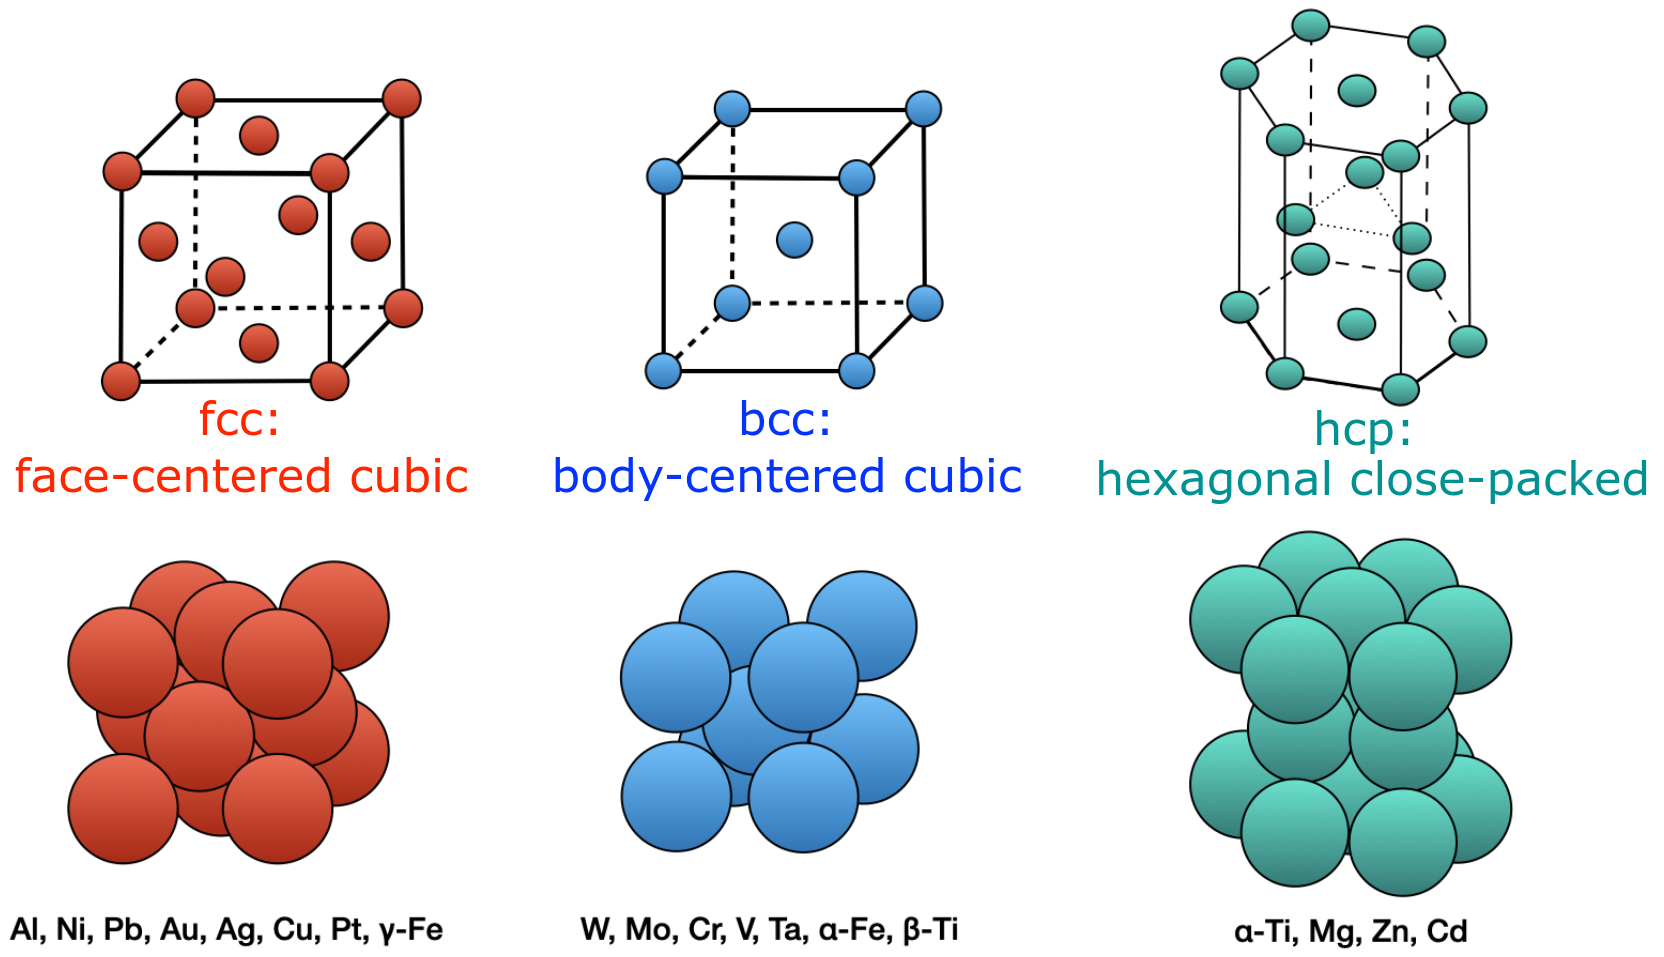
\includegraphics[width=0.71\textwidth]{media/fccbcchcp.png}
\end{center}

\begin{minipage}[t]{0.33\textwidth}
  \pph{FCC (Face-centered cubic)}
  \begin{itemize}
    \item Packing efficiency:\\[0.1cm]
      $\phi = \dfrac{\pi}{\sqrt{18}} \approx 74\%$
    \item Has many slip systems (12)
    \item Closest packed direction
  \end{itemize}
\end{minipage}%
\begin{minipage}[t]{0.33\textwidth}
  \pph{BCC (Body-centered cubic)}
  \begin{itemize}
    \item Packing efficiency:\\[0.1cm]
      $\phi = \dfrac{\sqrt{3\pi}}{8} \approx 68\%$
    \item Has many slip systems (6)
    \item Not closest packed direction
    \item Cottrell atmosphere
  \end{itemize}
\end{minipage}%
\begin{minipage}[t]{0.33\textwidth}
  \pph{HCP (Hexagonal close-packed)}
  \vspace*{-0.45cm}
  \begin{itemize}
    \item Packing efficiency:\\[0.1cm]
      $\phi = \dfrac{\pi}{\sqrt{18}} \approx 74\%$
    \item Very few slip systems (3)
    \item Closest packed direction
  \end{itemize}
\end{minipage}

\figbox{$\text{Packing efficiency}\, \left(\phi\right) = \dfrac{\text{Volume occupied by atoms in unit cell}}{\text{Total volume of unit cell}}$}
\newpage

\subsection{Structural model of ceramics}
In general, ceramics have:
\begin{itemize}
  \item \textbf{Ionic bonding, complex crystal structures (ceramics), amorphous (glasses)}
  \item Undoped: insulators (doped: semiconductors, superconductors or ionic conductors)
  \item Brittle, but high chemical and thermal resistance
  \item Wear-resistant, other special properties (e.g. ferro-/piezoelectricity)
\end{itemize}

\begin{figure*}[ht!]
  \centering
  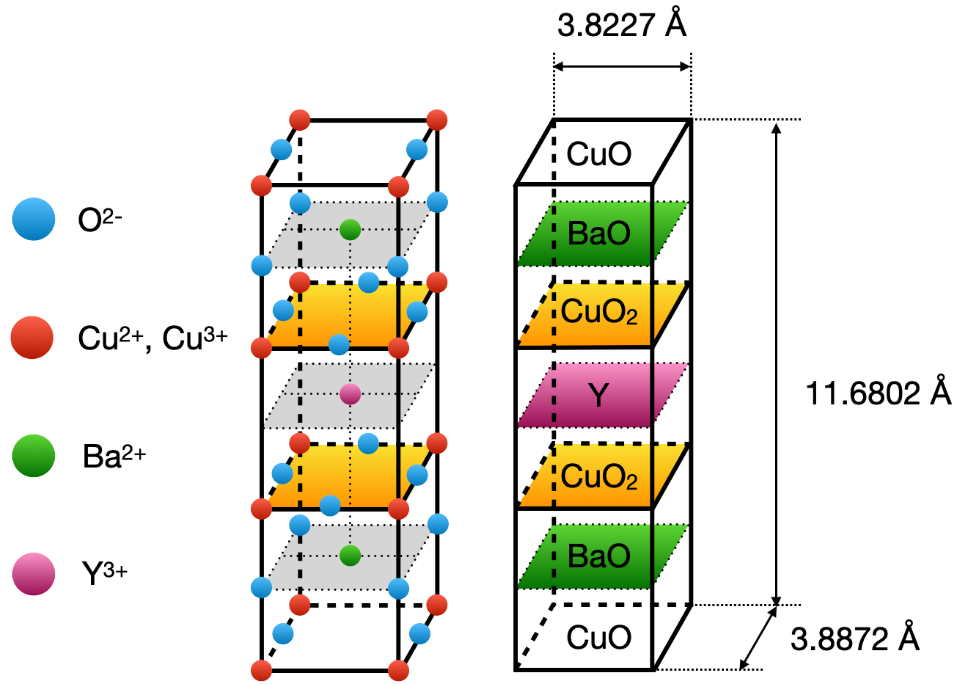
\includegraphics[width=0.6\textwidth]{media/ceramic_structure.png}
  \caption*{YBCO superconducting ceramic with layered perovskite-like structure}
\end{figure*}

\subsection{Structural model of polymers}
In general, polymers have:
\begin{itemize}
  \item Macromolecules ($10^3$ to $10^5$ C atoms)
  \item \textbf{Weaker intermolecular bonds} (strong atomic bond in molecular chain)
  \item Electrically and thermally insulating (without special modifications)
  \item Cheap, moldable, massive waste problem (e.g. ocean pollution)
  \item Matrix for many composite materials (recycling problem)
\end{itemize}
\begin{figure*}[ht!]
  \centering
  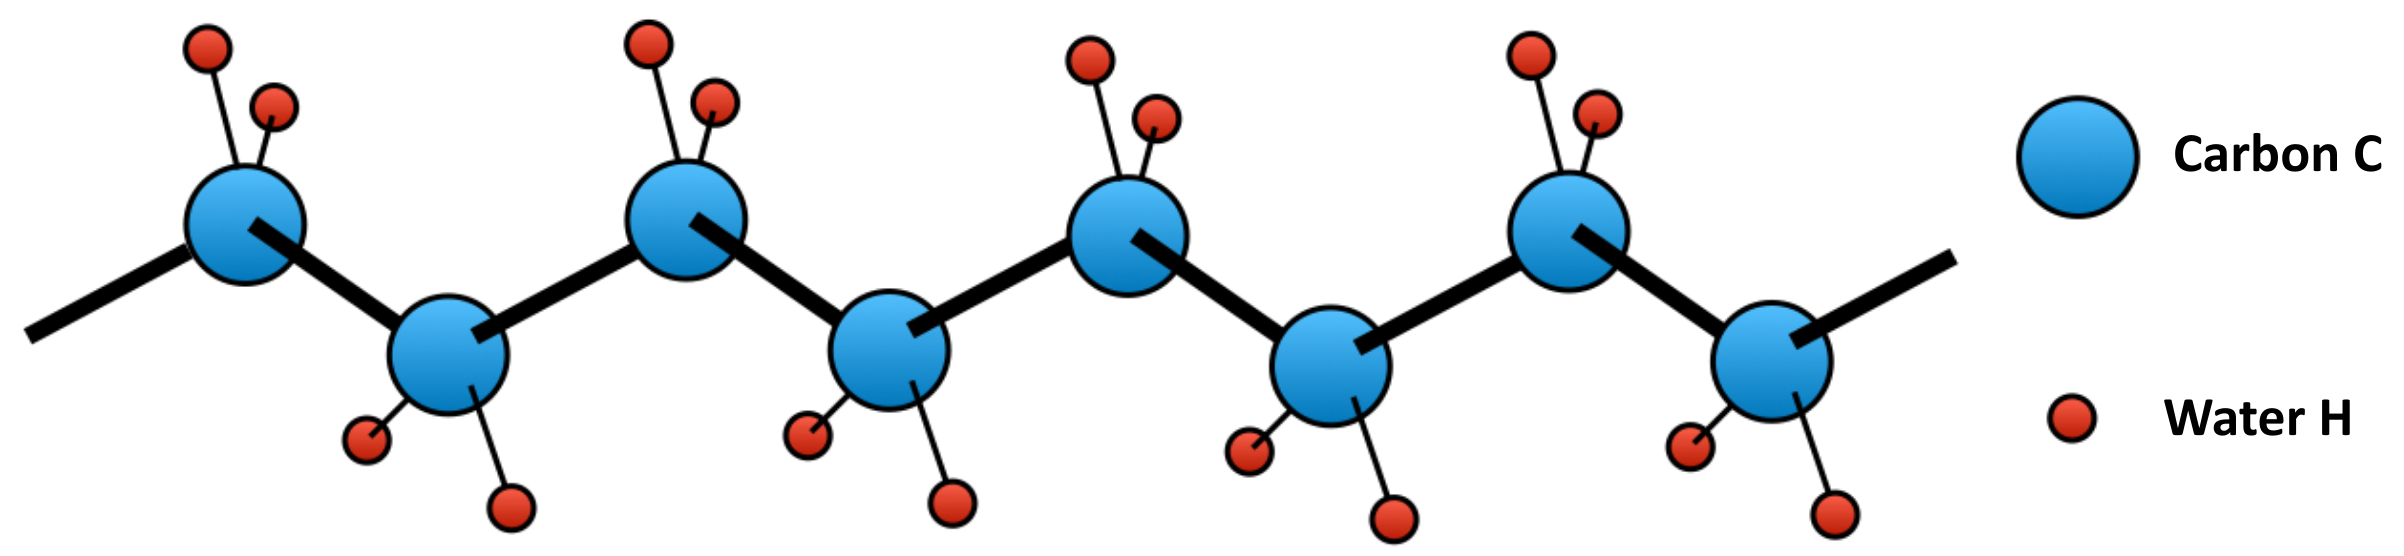
\includegraphics[width=0.8\textwidth]{media/polymer_structure.png}
  \caption*{Polymeric hydrocarbon chain}
\end{figure*}

\subsection{Amorphous and crystalline materials}
\begin{minipage}[t]{0.48\textwidth}
  \textbf{Amorphous materials}
  \begin{itemize}
    \item No crystal lattice (e.g. quartz glass, polymers)
    \item Atomic distances defined by chemical bonds
    \item Bond angles are variable
  \end{itemize}
\end{minipage}
\hfill
\begin{minipage}[t]{0.48\textwidth}
  \textbf{Crystalline materials}
  \begin{itemize}
    \item Crystal lattice (e.g. metals, ceramics, quartz)
    \item Atomic distances and bonding angles are defined
  \end{itemize}
\end{minipage}

\newpage
\begin{figure*}[ht!]
  \centering
  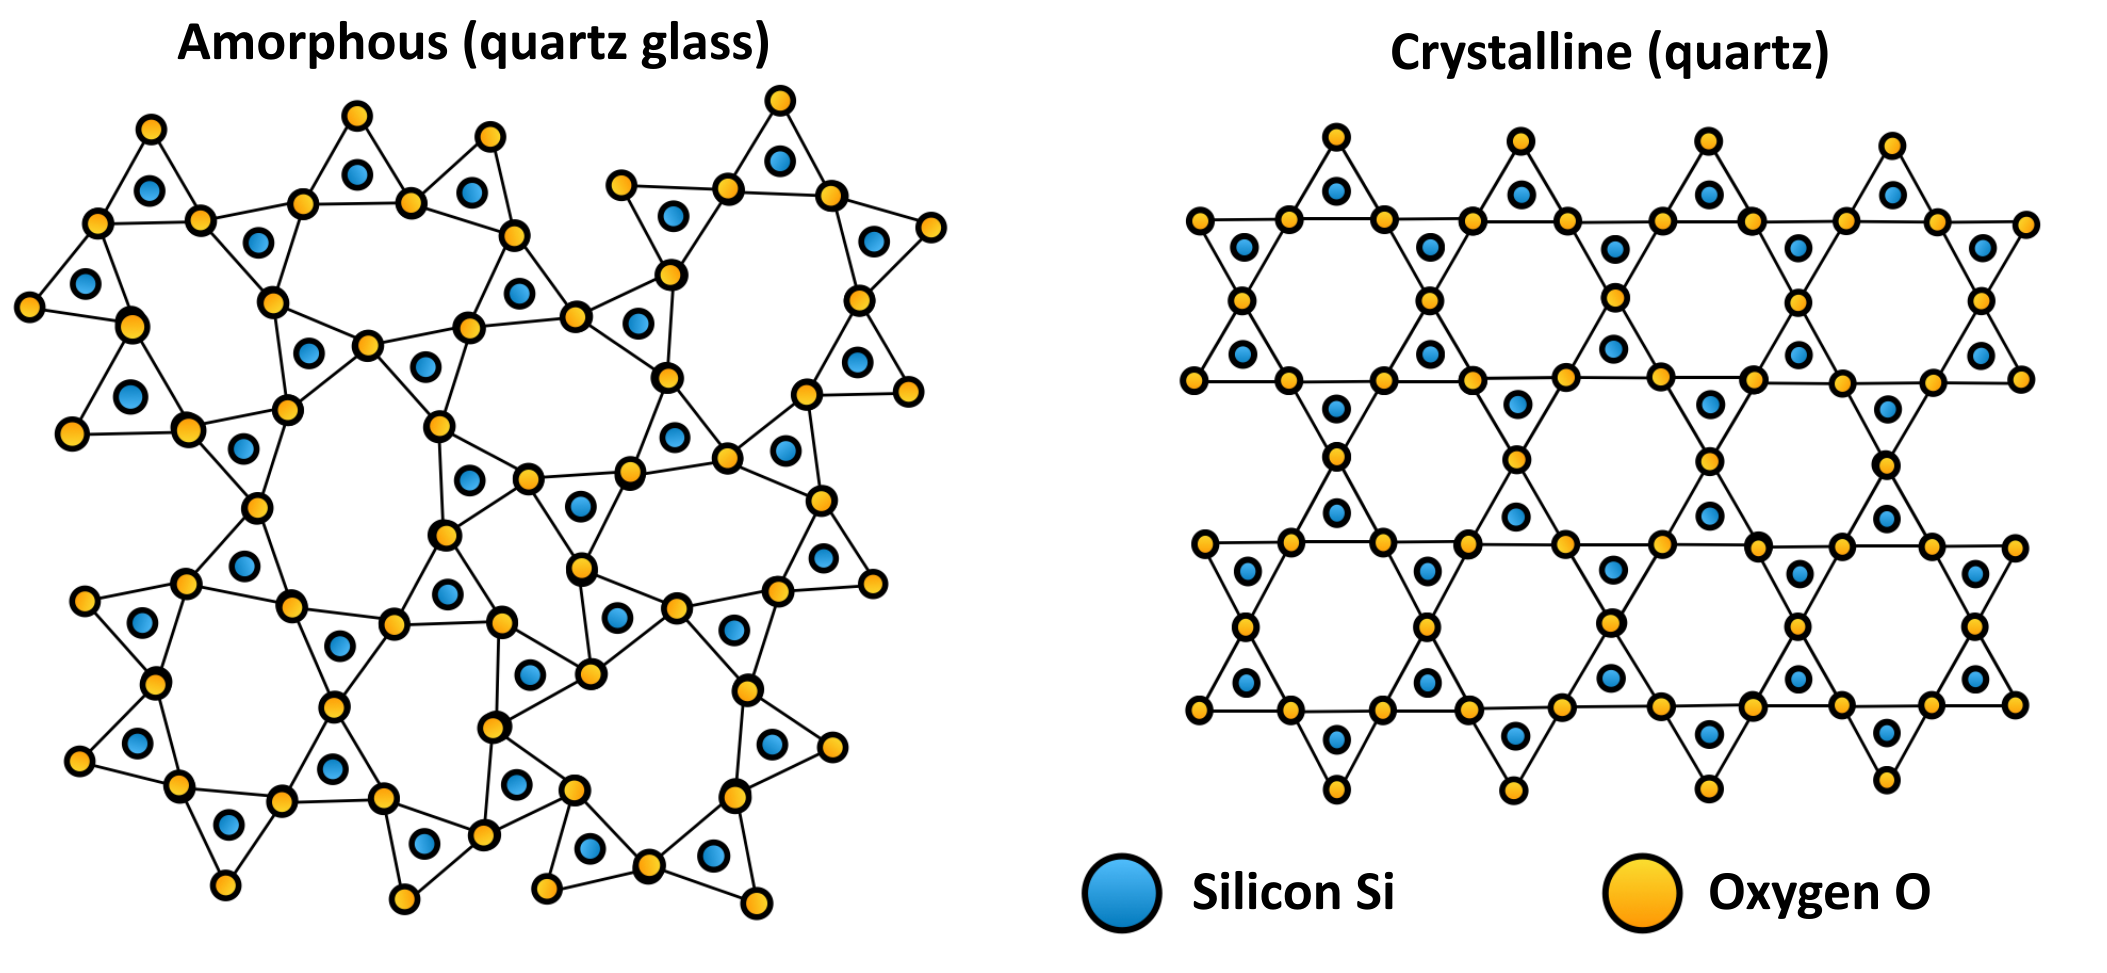
\includegraphics[width=0.8\textwidth]{media/amorph_cry.png}
\end{figure*}

\subsubsection{Polycrystalline materials}
Most metal components are polycrystalline (made of many grains/crystals),
i.e. they consist of countless microscopic crystals (crystallites, ``grains'').

\subsubsection{Monocrystalline materials}
\textbf{Only for special applications, expensive}
\begin{itemize}
  \item Single-crystal turbine blades ($T>1000^\circ C$, creep-resistant)
  \item Semiconductors, MEMS components made of silicon (e.g. gyroscopes in smartphones, accelerometers)
  \item Optical elements (e.g. laser crystals, $\lambda/4$ plates, crystals for frequency doubling of lasers)
\end{itemize}


\subsubsection{Amorphous materials}
\begin{itemize}
  \item Inorganic glasses (also Gorilla glass of smartphones)
  \item Metallic glasses (ferrous transformer sheet metal)
  \item Amorphous plastics (e.g. PMMA - plexiglass, COC, \dots)
\end{itemize}

\subsubsection{Structure difference}
\begin{figure*}[ht!]
  \centering
  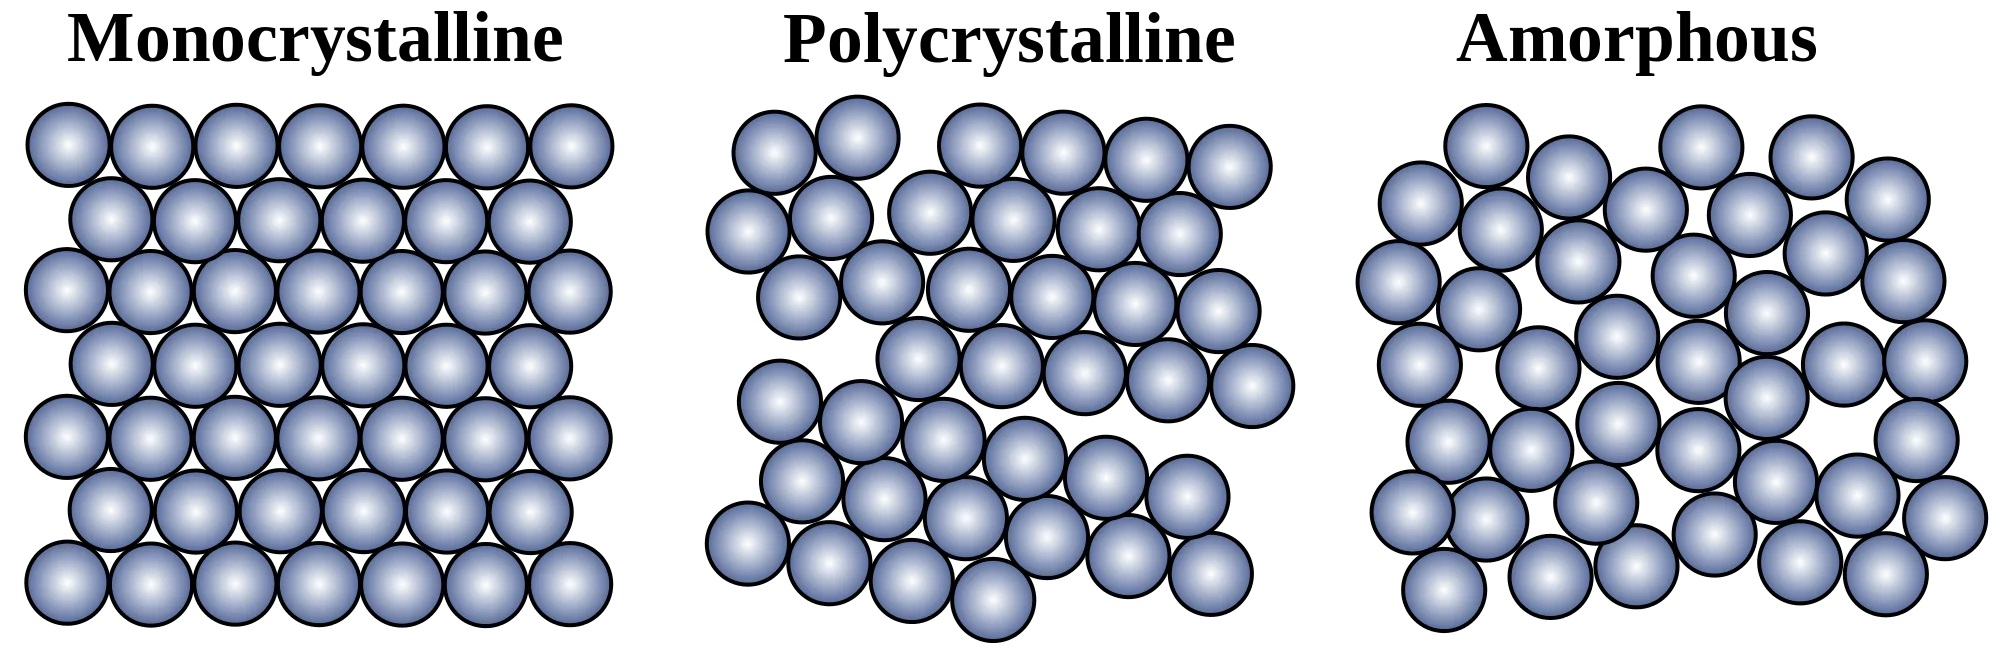
\includegraphics[width=0.8\textwidth]{media/mono_poly_amorph.jpg}
\end{figure*}

\subsection{Directionals dependence of the properties of materials}
\subsubsection{Anisotropy and Isotropy}
\begin{itemize}
  \item Anisotropic: Properties depend on direction (e.g. single crystals, wood, composites)
  \item Isotropic: Properties do not depend on direction (e.g. polycrystalline metals, amorphous materials)
\end{itemize}

\subsubsection{Anisotropy of the Young's Modulus $E$ in most cubic crystals}
In most cases, the $E$ is the largest in the direction of the closest packed atomic planes,
in direction of the space diagonal $\langle 111 \rangle$.

\newpage
\subsubsection{Miller indices for crystal directions}
In short, the Miller indices are the reciprocals of the fractional intercepts
that the plane makes with the crystallographic axes:
\begin{figure*}[ht!]
  \centering
  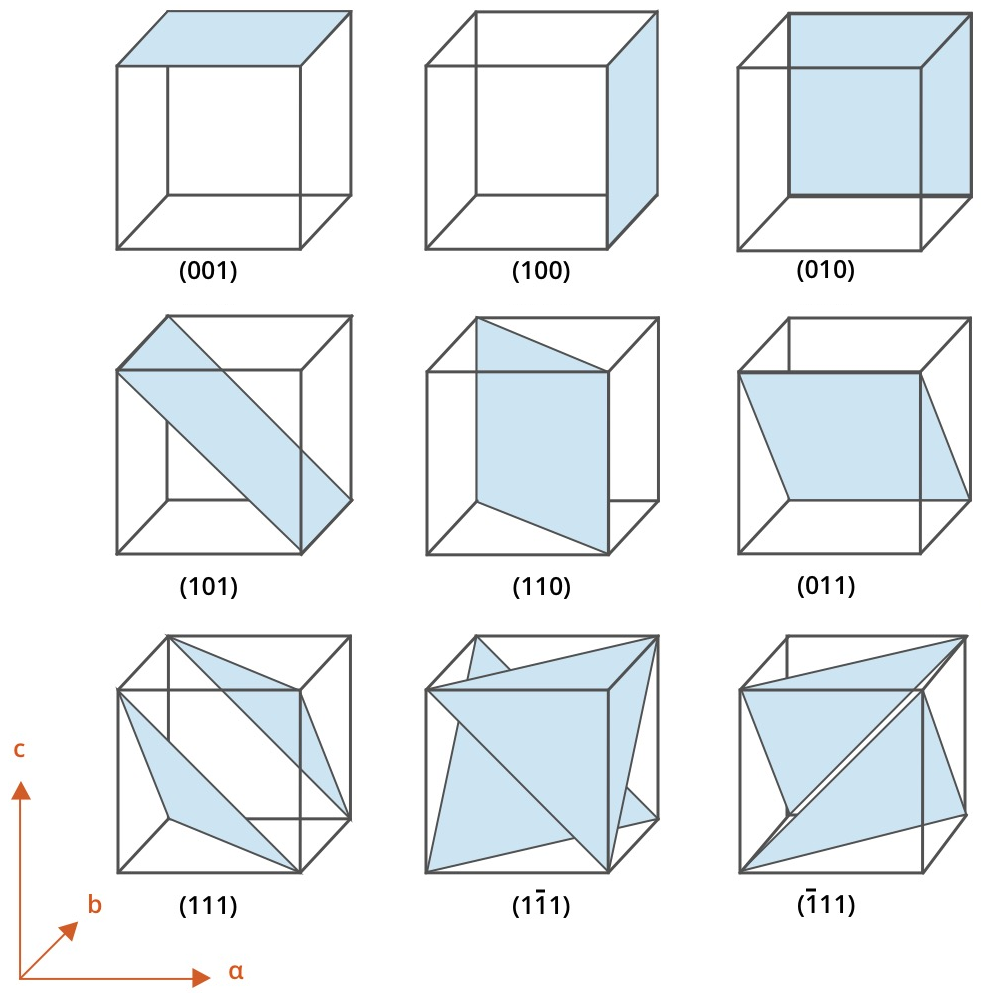
\includegraphics[width=0.5\textwidth]{media/miller_indices.png}
\end{figure*}

\subsection{Directional dependence of properties in polycrystalline materials}
\subsubsection{Polycrystalline materials without texture}
The polycrystalline materials without texture are considered \textbf{quasi-isotropic},
because the grains are randomly oriented.
\begin{figure*}[ht!]
  \centering
  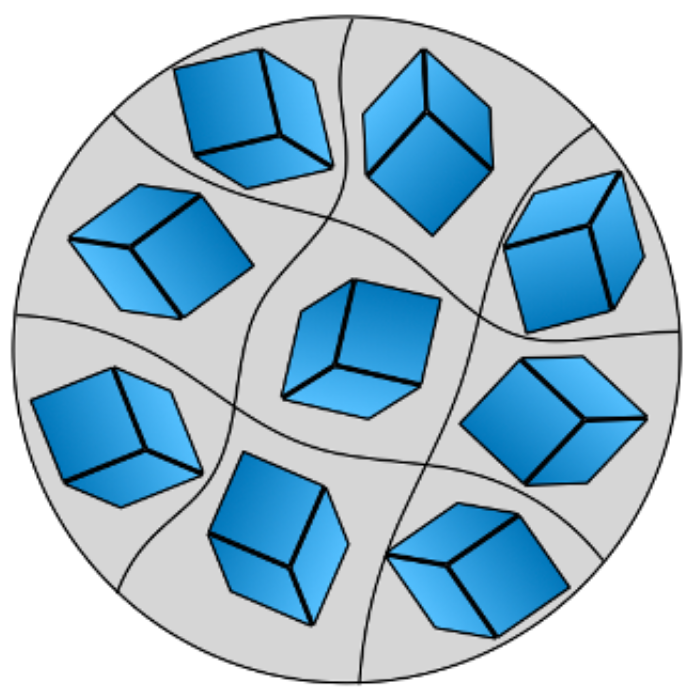
\includegraphics[width=0.1825\textwidth]{media/poly_notexture.png}
  \caption*{Polycrystalline material without texture}
\end{figure*}

\underline{Notice}: each crystal is anisotropic. but the material is quasi-isotropic to the outside, directional
dependence ``averages out''

\subsubsection{Polycrystalline materials with texture}
The polycrystalline materials with texture are considered \textbf{anisotropic},
because the grains are preferentially oriented.
\begin{figure*}[ht!]
  \centering
  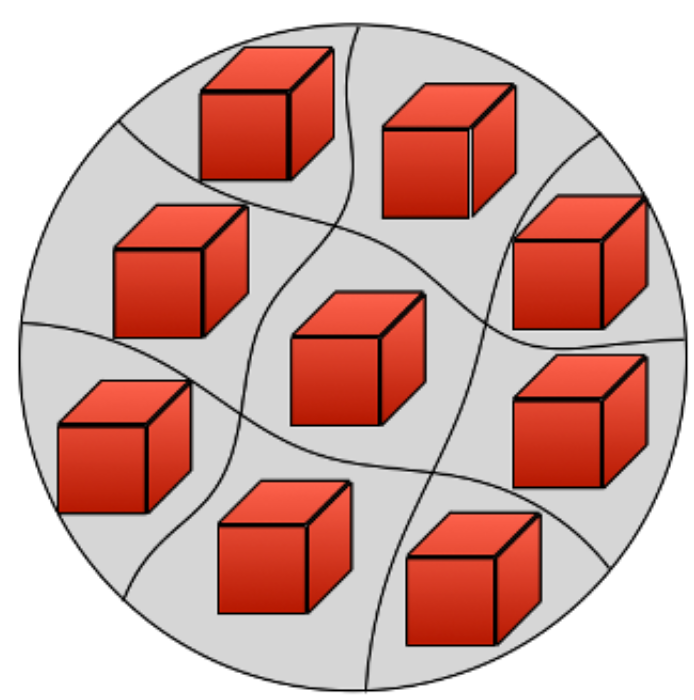
\includegraphics[width=0.1825\textwidth]{media/poly_texture.png}
  \caption*{Polycrystalline material with texture}
\end{figure*}
\newpage

\subsection{Material properties wrap-up}
\subsubsection{Single crystal materials}
\begin{itemize}
  \item \textbf{Anisotropic}
  \item Properties depend on direction
  \item Not uniform = anisotropic
\end{itemize}

\subsubsection{Polycrystalline materials without texture}
\begin{itemize}
  \item \textbf{Quasi-isotropic}
  \item Each crystal: anisotropic
  \item Uniform properties in all directions: isotropic \textrightarrow\ quasi-isotropic
\end{itemize}

\subsubsection{Polycrystalline materials with texture}
\begin{itemize}
  \item \textbf{Anisotropic}
  \item Preferential orientation of the crystallites: texture \textrightarrow\ anisotropic
  \item Examples: rolled and recrystallized electrical sheets with Goss texture
\end{itemize}

\subsubsection{Amorphous materials}
\begin{itemize}
  \item \textbf{Isotropic} (e.g. glass or amorphous metals)
\end{itemize}

\subsection{Polymorphism (Allotropy)}
Some materials may exhibit more than one crystal structure:
\begin{itemize}
  \item Iron $
    \begin{cases}
      \alpha\text{-Fe (ferrite, BCC)} & \text{below } 911^\circ\text{C} \\
      \gamma\text{-Fe (austenite, FCC)} & 911^\circ\text{C} \text{ to } 1392^\circ\text{C} \\
      \delta\text{-Fe (ferrite, BCC)} & 1392^\circ\text{C} \text{ to } 1536^\circ\text{C}
    \end{cases}$
  \item Titanium $
    \begin{cases}
      \text{HCP} & \text{below } 880^\circ\text{C} \\
      \text{BCC} & \text{above } 880^\circ\text{C}
    \end{cases}$
  \item Shape memory alloys (e.g. NiTi)
  \item Carbon (graphite, diamond, graphene, fullerene, CNT, \dots)
  \item Zirconia (high crack resistance due to phase transformation toughening)
  \item Ferro- and piezoelectric materials (e.g. PZT, quartz, \dots)
\end{itemize}

\subsubsection{Polymorphism of Iron (Fe)}
\begin{figure}[ht!]
\centering
\begin{minipage}[t]{0.48\textwidth}
  \centering
  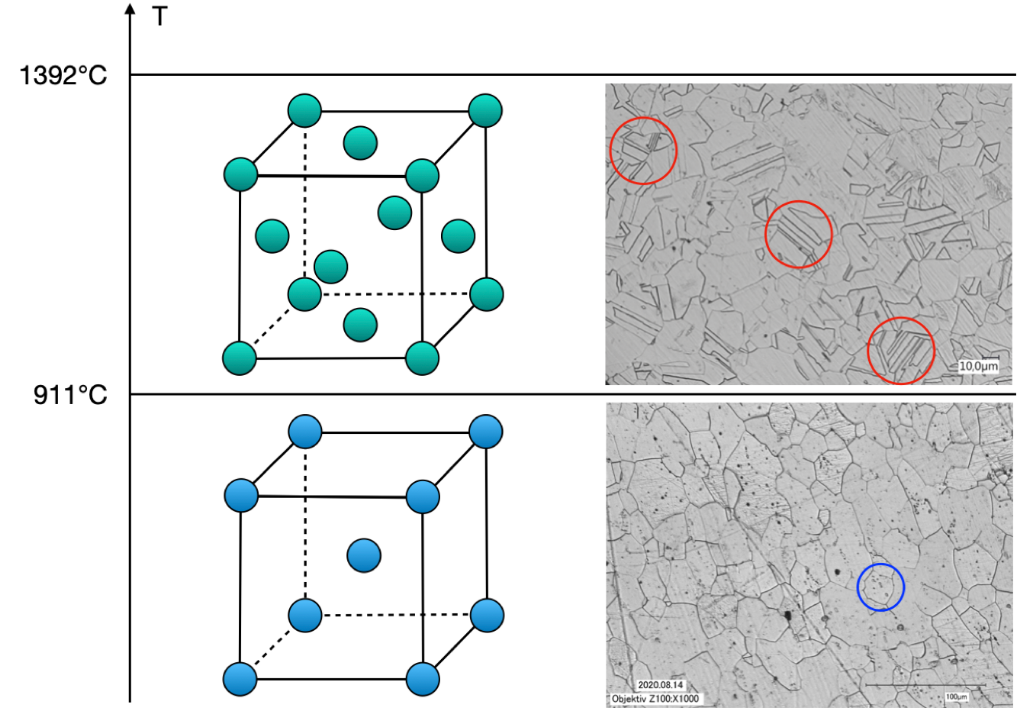
\includegraphics[width=\linewidth]{media/ferrite_trans.png}
  \captionof*{figure}{Slow Austenite transformation in steel: Ferrite}
\end{minipage}\hfill
\begin{minipage}[t]{0.48\textwidth}
  \centering
  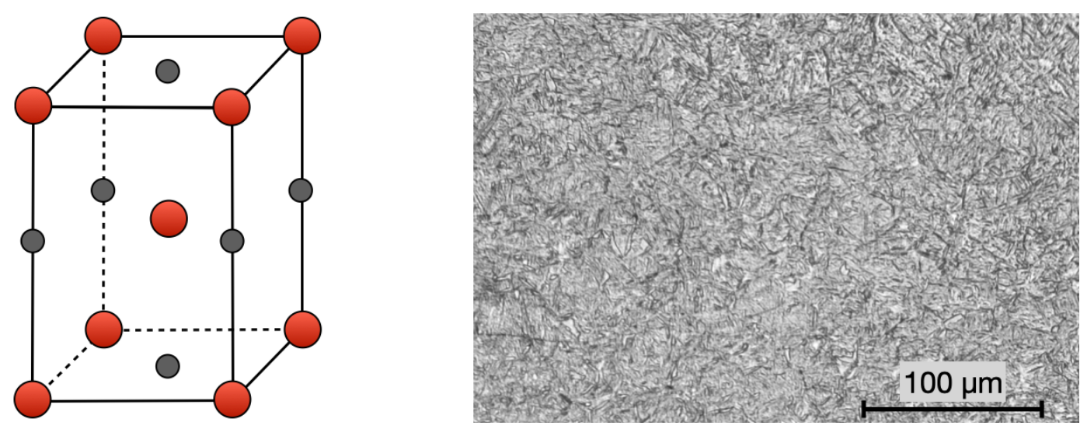
\includegraphics[width=\linewidth]{media/martenesite_trans.png}
  \captionof*{figure}{Fast Austenite transformation: Martensite}
\end{minipage}
\end{figure}

\newpage
\subsubsection{Polymorphism of Carbon (C)}
\forestset{
  mybox/.style={
    draw, rounded corners, align=center, inner sep=4pt, outer sep=2pt
  },
  my edge/.style={-latex}
}

\begin{forest}
for tree={
  mybox,
  edge={-latex},
  l sep=10pt,
  s sep=8pt,
  anchor=north
}
[Carbon
  [Amorphous Carbon
    [Activated Carbon]
    [Templated Carbon]
  ]
  [Crystalline Carbon
    [Graphite
      [Paracrystalline]
      [Rhombic]
      [Hexagonal]
    ]
    [Fullerene]
    [CNT]
    [Carbyne]
    [Diamond
      [Cubic]
      [Hexagonal]
    ]
  ]
]
\end{forest}

\subsubsection{Polymorphism of Nitinol (NiTi)}
NiTi is a shape memory alloy (SMA), used for screen lock of tablet notebooks, medtech,
and spectacle frames.
\begin{figure*}[ht!]
  \centering
  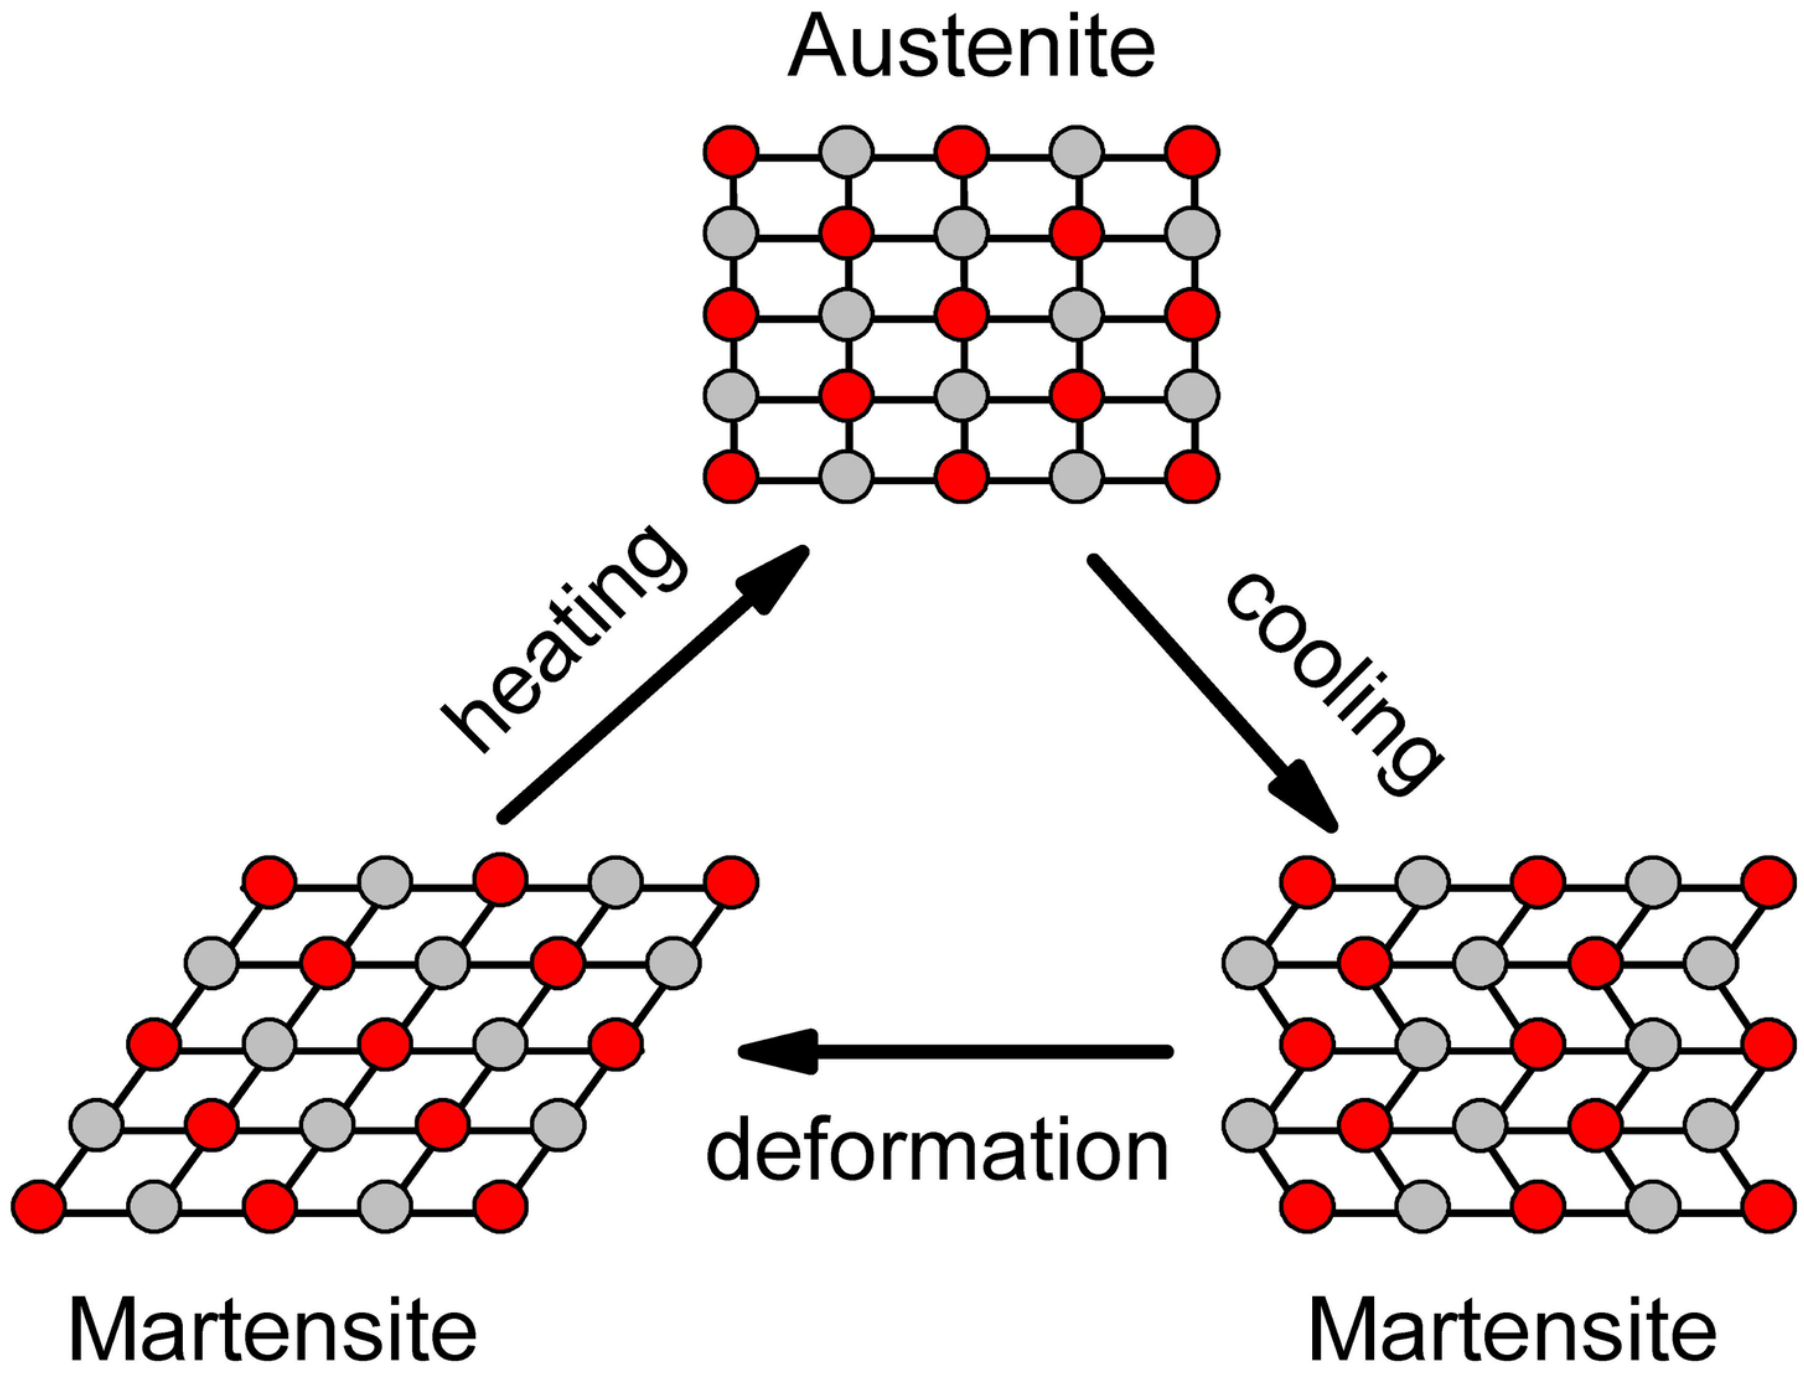
\includegraphics[width=0.4\textwidth]{media/Nitinol.png}
\end{figure*}

\subsection{Microstructure and Phases}
Phases are \textbf{homogeneous} subsections of a material with uniform physical and chemical properties:
\begin{itemize}
  \item A phase can be crystalline or amorphous
  \item At the phase boundaries, a sudden change in structure, properties and chemical composition occurs
\end{itemize}

Polycristalline materials can consist of:
\begin{itemize}
  \item One phase (homogeneous microstructure, e.g. only iron crystals)
  \item Different phases (heterogeneous microstructure, e.g. graphite and iron)
\end{itemize}

\begin{minipage}[t]{0.48\textwidth}
  \subsubsection{Homogeneous microstructure}
  They have only one phase and crystal structure:
  \vspace*{0.8cm}
  \begin{center}
    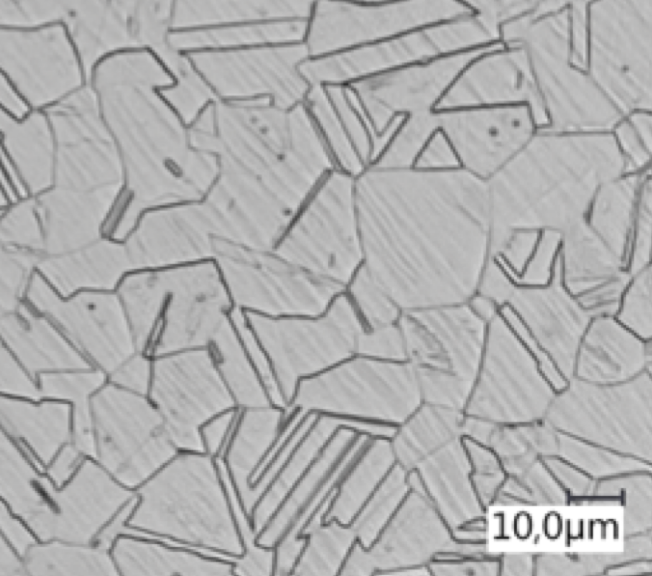
\includegraphics[width=0.65\textwidth]{media/homogeneous_microstructure.png}
  \end{center}
\end{minipage}
\hfill
\begin{minipage}[t]{0.48\textwidth}
  \subsubsection{Heterogeneous microstructure}
  They have multiple phases and many types of crystal structures:
  \vspace*{0.5cm}
  \begin{center}
    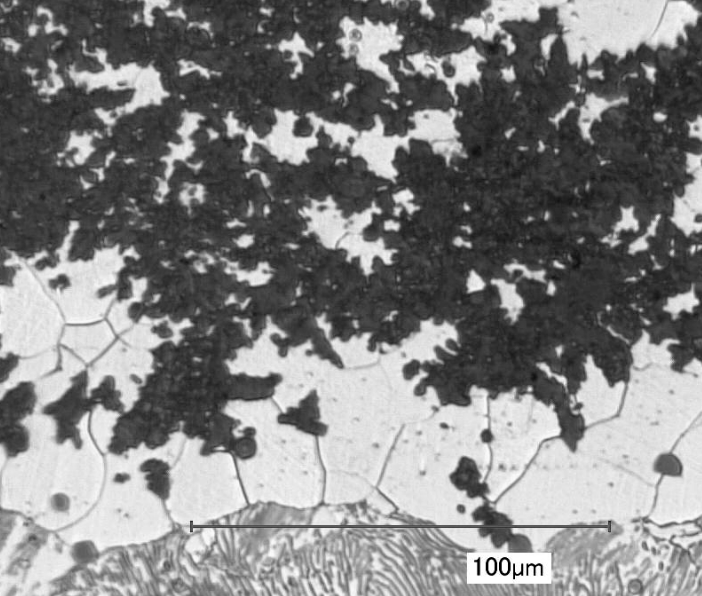
\includegraphics[width=0.7\textwidth]{media/heterogeneous_microstructure.png}
  \end{center}
\end{minipage}

\newpage
\subsection{Alloys}
\subsubsection{Definition of an alloy}
An alloy is a metallic material of at least 2 types of atoms:
\begin{itemize}
  \item Metal + Metal (iron-nickel, gold-silver, tin-lead, aluminum-copper, \dots)
  \item Metal + Non-metal (iron-carbon (steel), nickel-phosphorus, \dots)
\end{itemize}

\subsubsection{Microstructure of alloys}
\begin{itemize}
  \item \textbf{Homogeneous}, single-phase, only one type of cristal: SOLID SOLUTION CRYSTAL
  \item \textbf{Heterogeneous}, multi-phase, MIX OF DIFFERENT CRYSTAL TYPES:
  \begin{itemize}
    \item Crystals of pure metals without impurity atoms (no solid solution crystals)
    \item Solid solution crystals with impurity atoms,
    \item Crystals of intermetallic or intermediate phases (chem compounds crystals with their own distinguished crystal structure e.g. Ni$_3$Ti, Fe$_3$C, \dots)
    \item (Impurity particles, e.g. added ceramic particles or slag residues)
  \end{itemize}
\end{itemize}

\section{Most important metal structures and crystal lattice defects}
\subsection{Lattice defects}
Lattice defects are irregularities in the crystal structure:
\begin{itemize}
  \item \textbf{0-dimensional defects} (point defects)
  \item \textbf{1-dimensional defects} (line defects)
  \item \textbf{2-dimensional defects} (surface defects)
  \item \textbf{3-dimensional defects} (volume defects)
\end{itemize}

\subsubsection{0-dimensional defect}
0-dimensional defects include vacancies (missing atoms) and impurity atoms (foreign atoms in the lattice).

The approximate atomic size is 0.1nm.

\begin{figure*}[ht!]
  \centering
  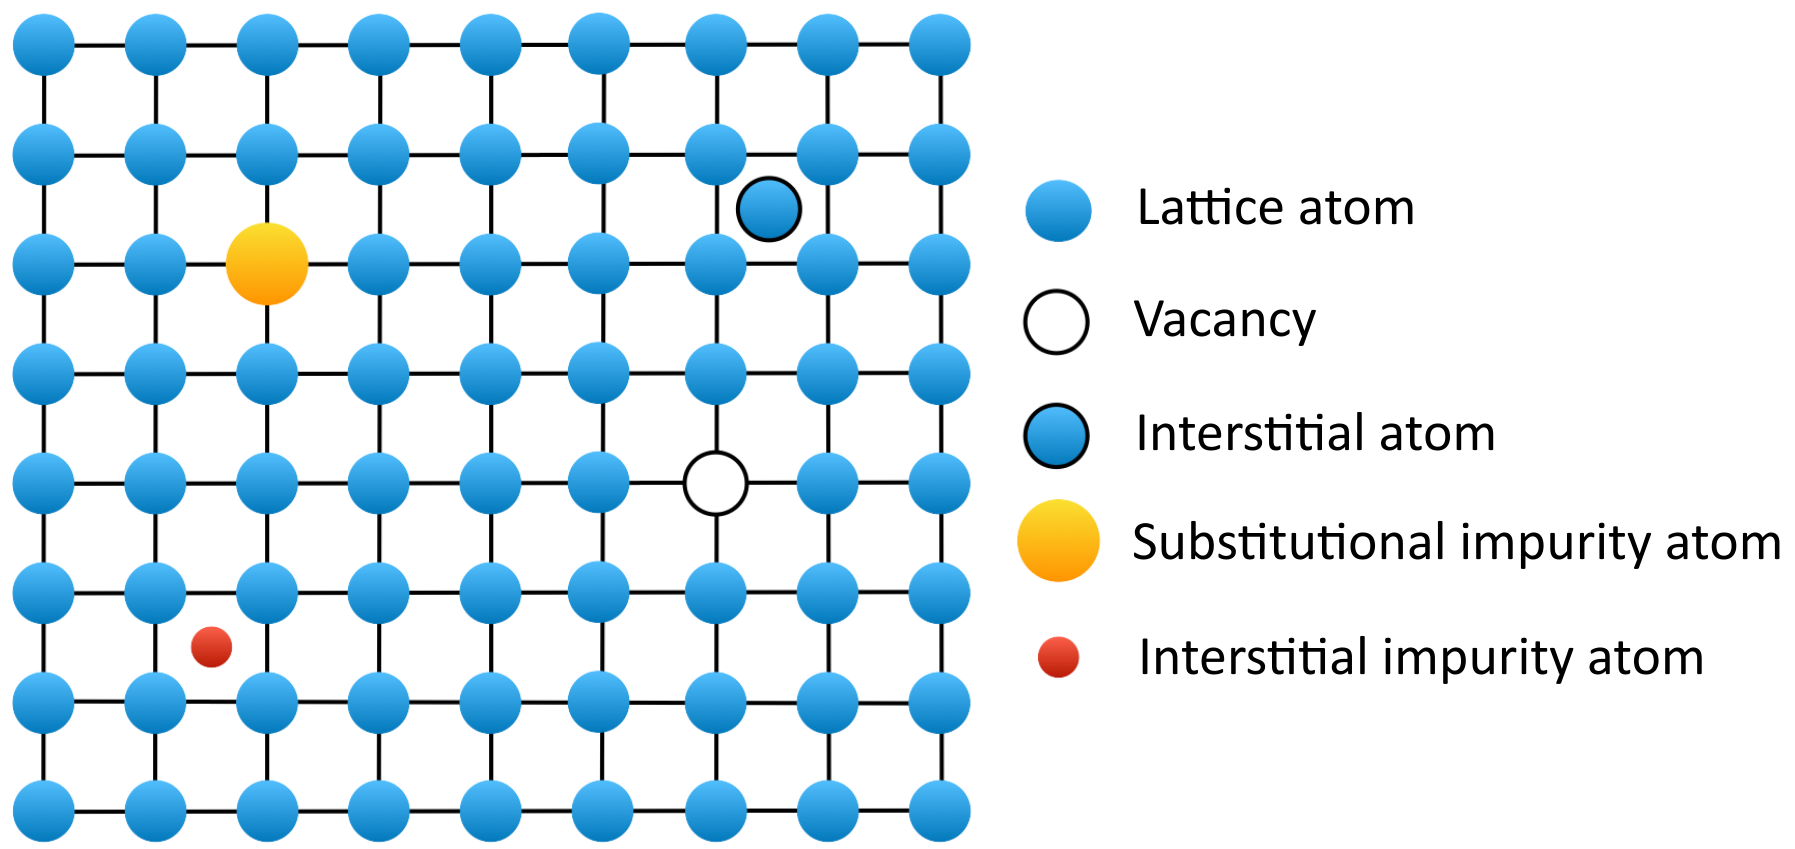
\includegraphics[width=0.6\textwidth]{media/lattice_0d.png}
  \caption*{Point defects: vacancy, interstitial atom, substitutional atom}
\end{figure*}

\newpage
\subsubsection{1-dimensional defect}
1-dimensional defects are dislocations (line defects) in the crystal structure.

Edge dislocations insert an extra half-plane of atoms in the crystal,
distorting the nearby planes of atoms.

\begin{figure*}[ht!]
  \centering
  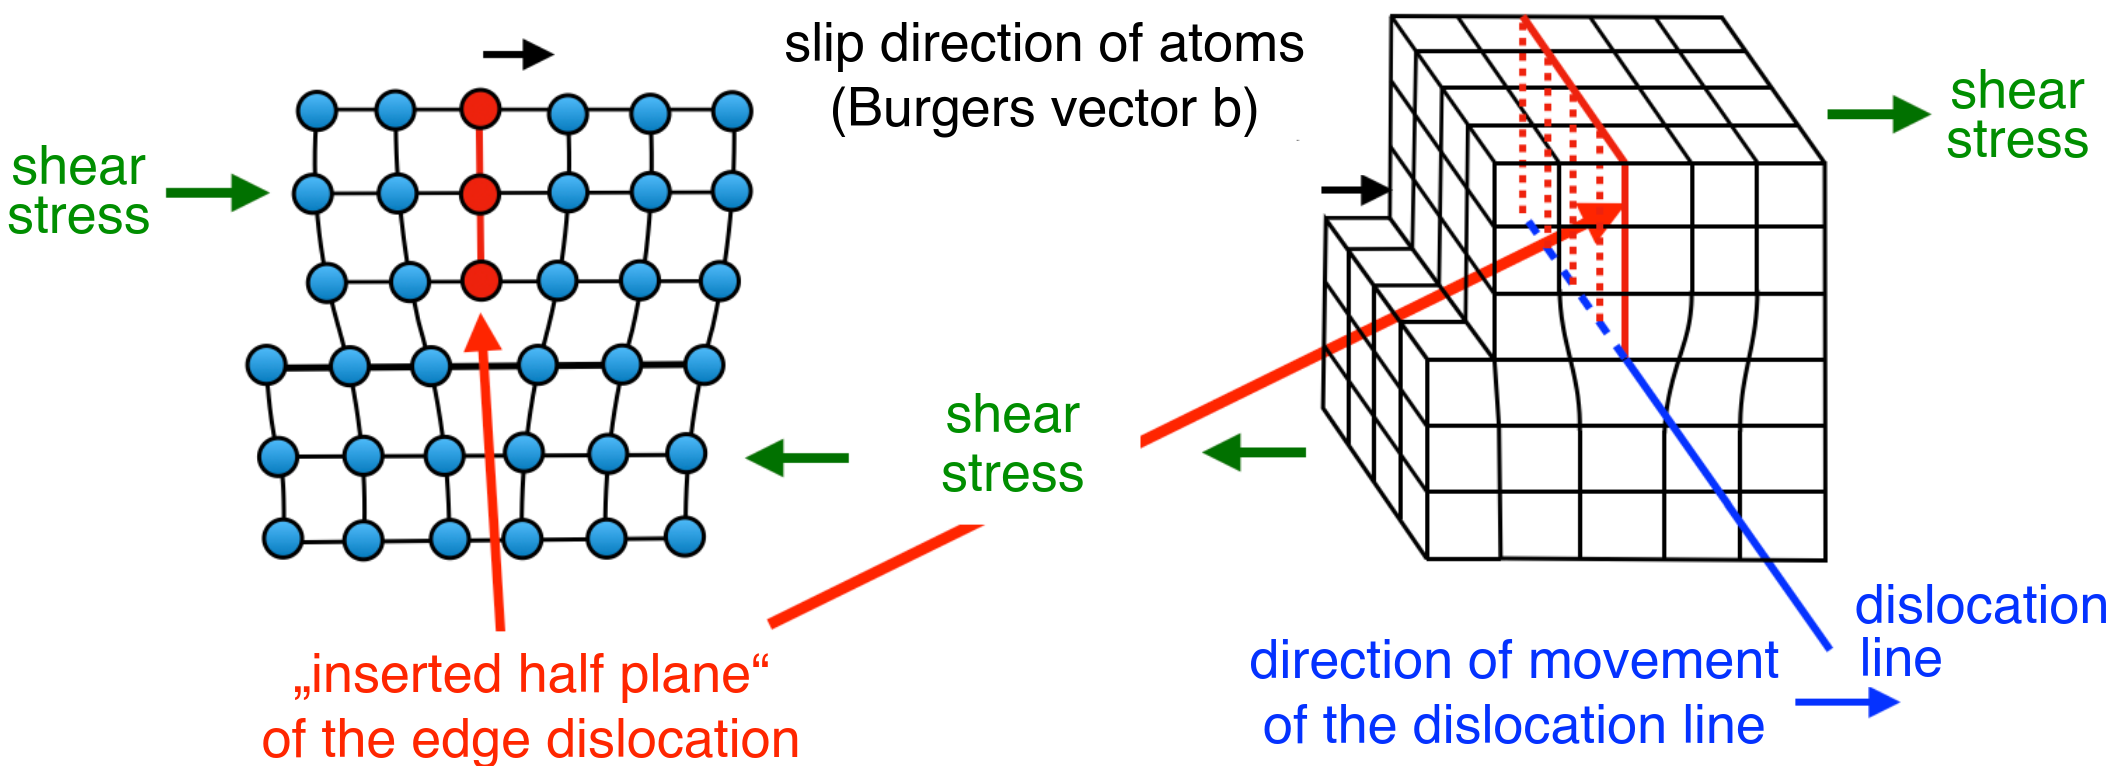
\includegraphics[width=0.8\textwidth]{media/lattice_1d.png}
  \caption*{Line defects: edge dislocation, screw dislocation}
\end{figure*}

\subsubsection{2-dimensional defect}
2-dimensional defects are grain boundaries (surface defects) in polycrystalline materials:
\begin{itemize}
  \item Crystal growth starts at multiple locations within the molten metal.
  \item Finally, the growing grains merge to form the microstructure of the solid metal.
\end{itemize}

The approximate atomic size is 10 to 100 $\mu$m.

\begin{figure*}[ht!]
  \centering
  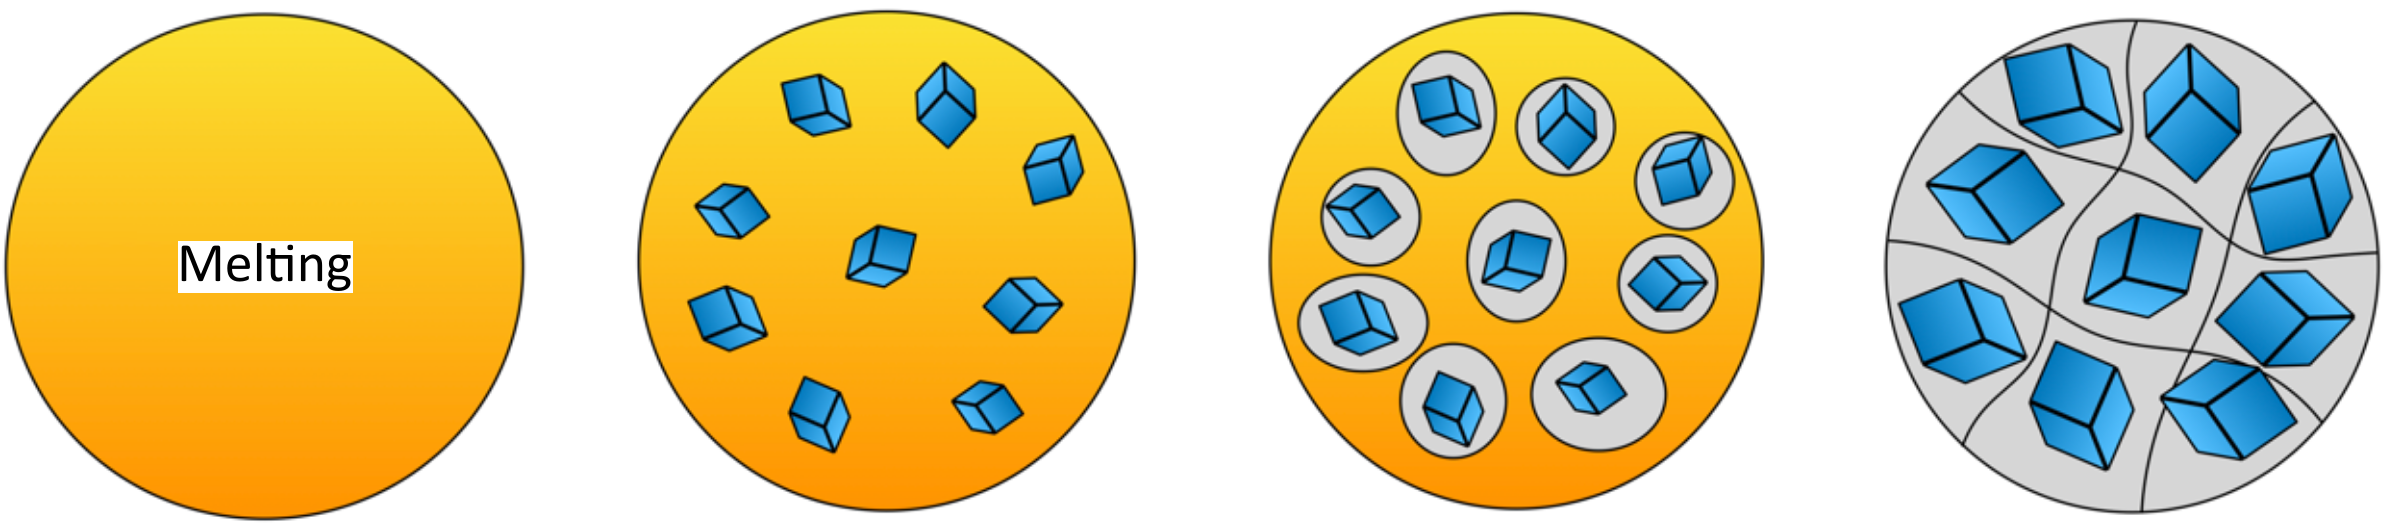
\includegraphics[width=0.8\textwidth]{media/lattice_2d.png}
  \caption*{Crystallization from a melt:\\(1) homogeneous melt, (2) nucleation of crystals, (3) crystal growth surrounded by residual melt, (4) fully solidified polycrystalline structure with grain boundaries}
\end{figure*}

\subsubsection{3-dimensional defect}
3-dimensional defects are precipitates, inclusions, voids, cracks (volume defects) in the crystal structure.

The size is very small (nanometers)
\begin{figure*}[ht!]
  \centering
  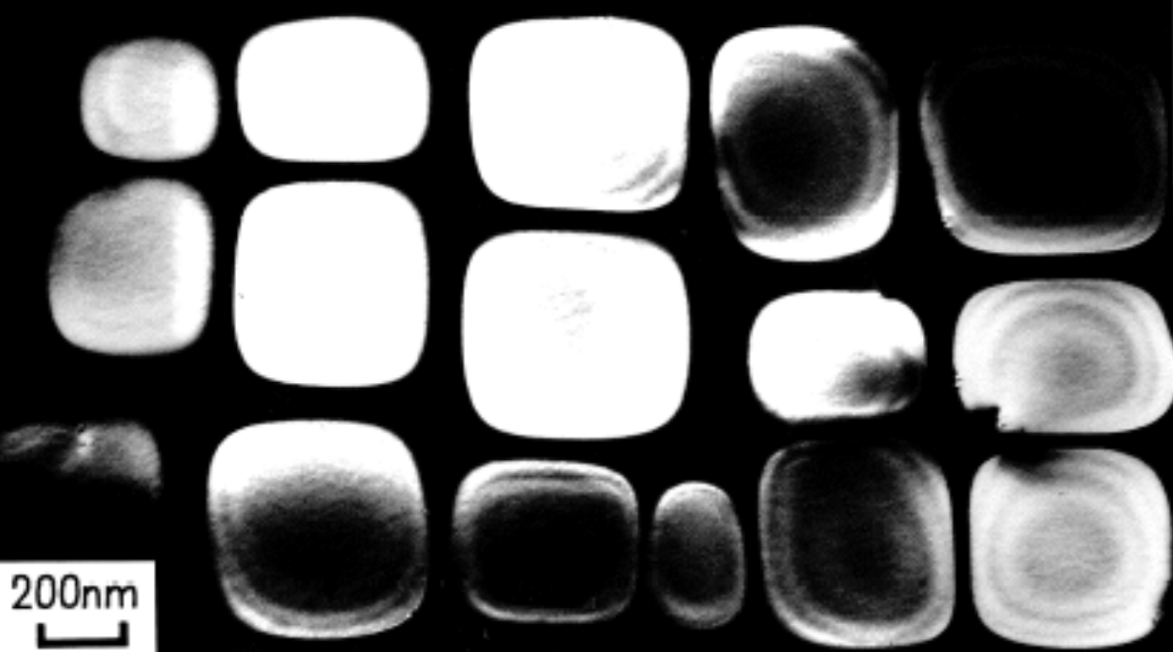
\includegraphics[width=0.55\textwidth]{media/lattice_3d.png}
  \caption*{Coherent Ni$_3$Al precipitates (white) in a Ni solid solution crystal (black)}
\end{figure*}

\newpage
\begin{wrapfigure}{l}{0.55\textwidth}
  \section{Elastic and plastic deformation}
  \subsection{Elastic deformation}
  \subsubsection{Atomic energy-distance model}
  The atomic energy-distance model describes the interaction between two atoms.

  The coefficient of thermal expansion $\alpha$ is inversely proportional to:
  \begin{itemize}
    \item Young's modulus $E$ (in case of springs, the force)
    \item Bonding energy
    \item Melting temperature
  \end{itemize}
\end{wrapfigure}

\phantom{}

\begin{figure*}[ht!]
  \begin{flushright}
    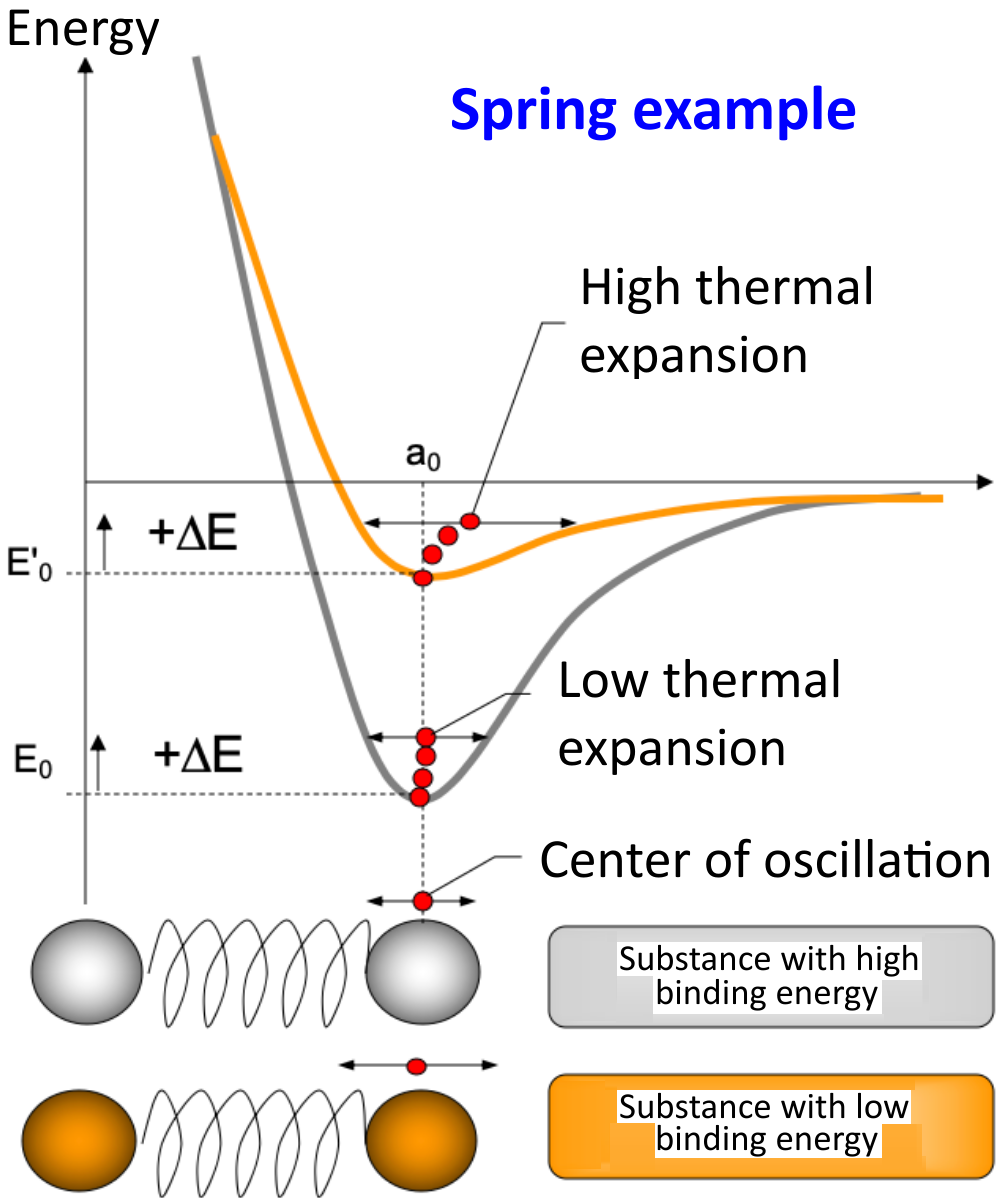
\includegraphics[width=0.4\textwidth]{media/atomic_energy_distance.png}
  \end{flushright}
\end{figure*}
\wrapfill

\vspace*{-8.6cm}

\subsection{Elastic constants of isotropic materials}
\subsubsection{Elastic stress, strain, and Young's modulus}
Letting the load be unidirectional and in x-direction, then:
\figbox{$\varepsilon_x = \dfrac{1}{E}\cdot \sigma_x\ \Longleftrightarrow\ \sigma_x = E \cdot \varepsilon_x$}

\subsubsection{Poisson's ratio $\nu$}
When a material is stretched in one direction (x-direction), it tends to contract in the other two directions (y- and z-directions).

The ratio of the transverse strain to the axial strain is called Poisson's ratio:
\figbox{$\nu = -\dfrac{\varepsilon_y}{\varepsilon_x} = -\dfrac{\varepsilon_z}{\varepsilon_x}$}

\subsubsection{Relationship between the 3 isotropic elastic constants $G$}
For isotropic materials, the following relationships hold:
\figbox{$G = \dfrac{E}{2(1+\nu)} = \dfrac{\sigma_x}{2\varepsilon_x(1+\nu)}$}

\subsection{Plastic deformation in metals}
The plastic deformation has as characteristics to be permanent and non-reversible.

\subsubsection{At room temperature}
\begin{itemize}
  \item Dislocations move on densely packed slip planes in densely packed directions
  \item Smaller slip distances require less external force or energy
\end{itemize}

\underline{Note}: There are exceptions. For example, metals with relatively low stacking
fault energy show:
\begin{itemize}
  \item Twin formation (e.g. nitinol)
  \item Partial dislocations pairs with stacking faults in between (e.g. Ni, Cu)
\end{itemize}

\subsubsection{At high temperatures}
The metal creeps, leading to diffusion of atoms, especially at grain boundaries.

\newpage
\subsection{Dislocation Slip Model}
The dislocation slip model describes the plastic deformation of metals by dislocation motion.

\subsubsection{Simplified model}
The simplified dislocation slip model is sufficient for practical understanding of plastic deformation:
\begin{itemize}
  \item Inserted half-plane, the end of which forms the dislocation line
  \item Dislocation moves on densely packed slip planes
\end{itemize}

\begin{figure*}[ht!]
  \centering
  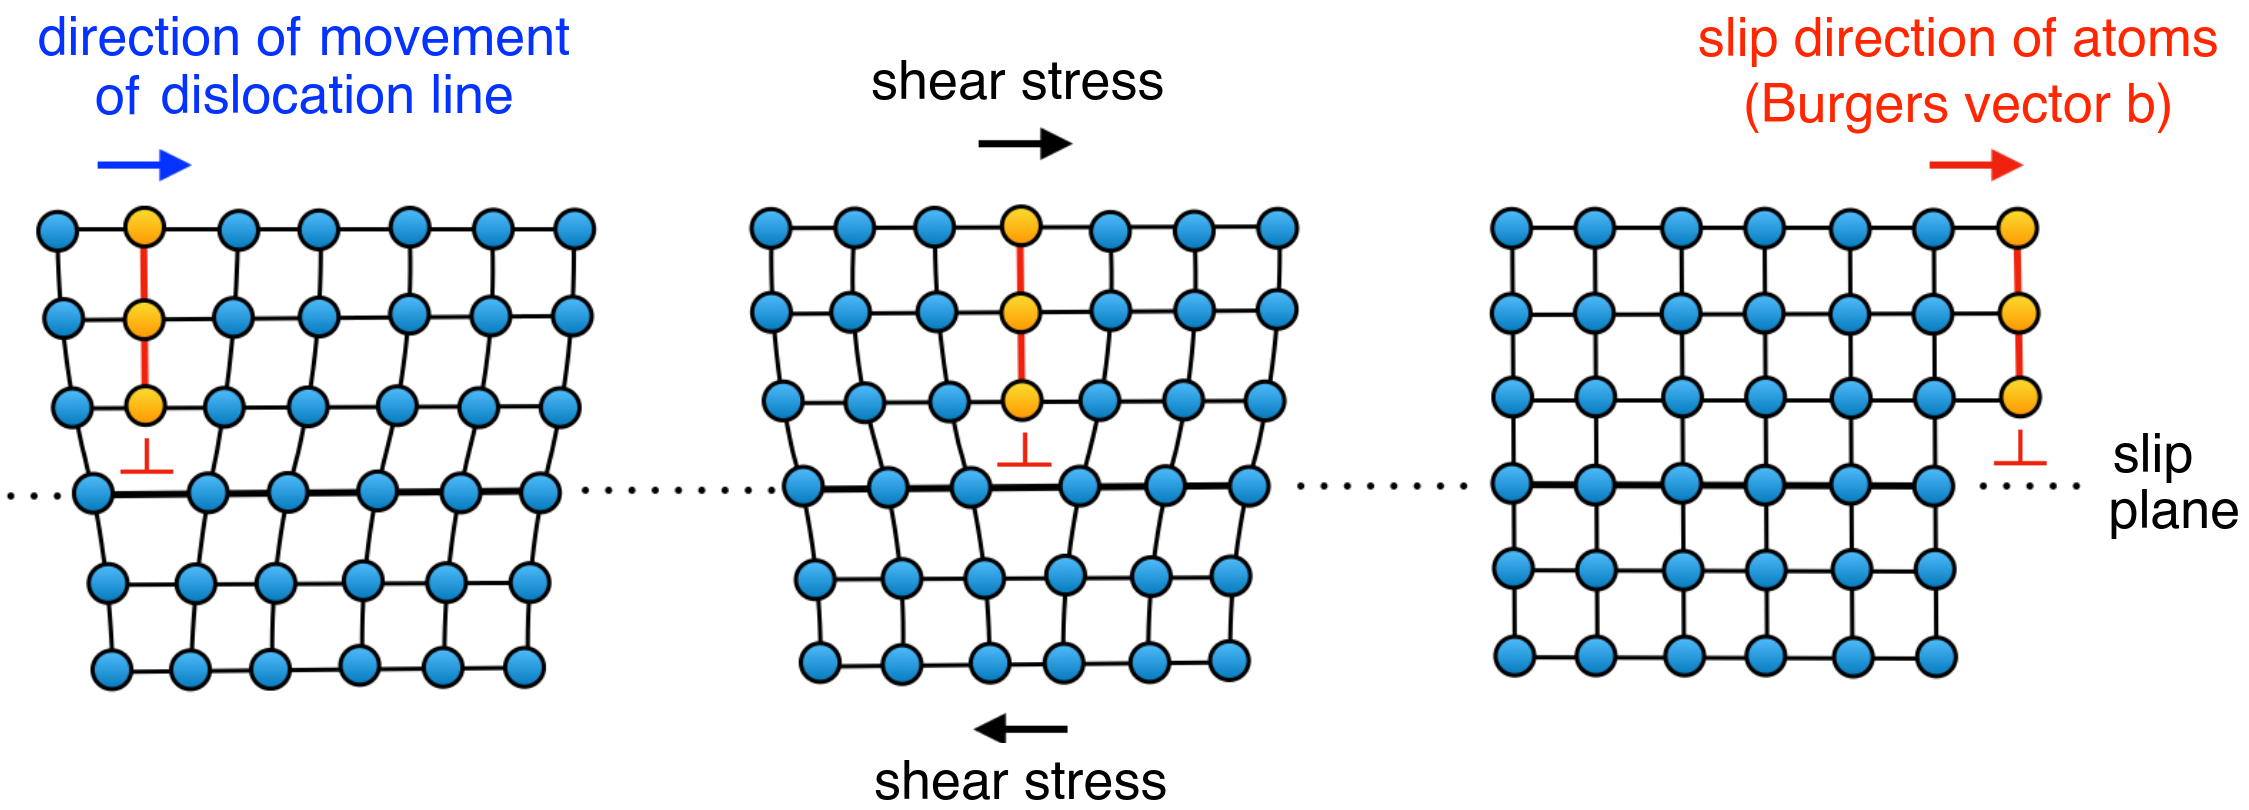
\includegraphics[width=0.8\textwidth]{media/simplified_dislocation_slip_model.png}
  \caption*{Edge dislocation motion under shear stress}
\end{figure*}

\subsection{Slip systems}
\subsubsection{Slip systems in FCC metals (Miller indices)}
FCC metals have 12 close-packed slip systems, making them soft and highly ductile (e.g. Au, Ag, Cu, Al, $\alpha$-Fe)
\begin{figure*}[ht!]
  \centering
  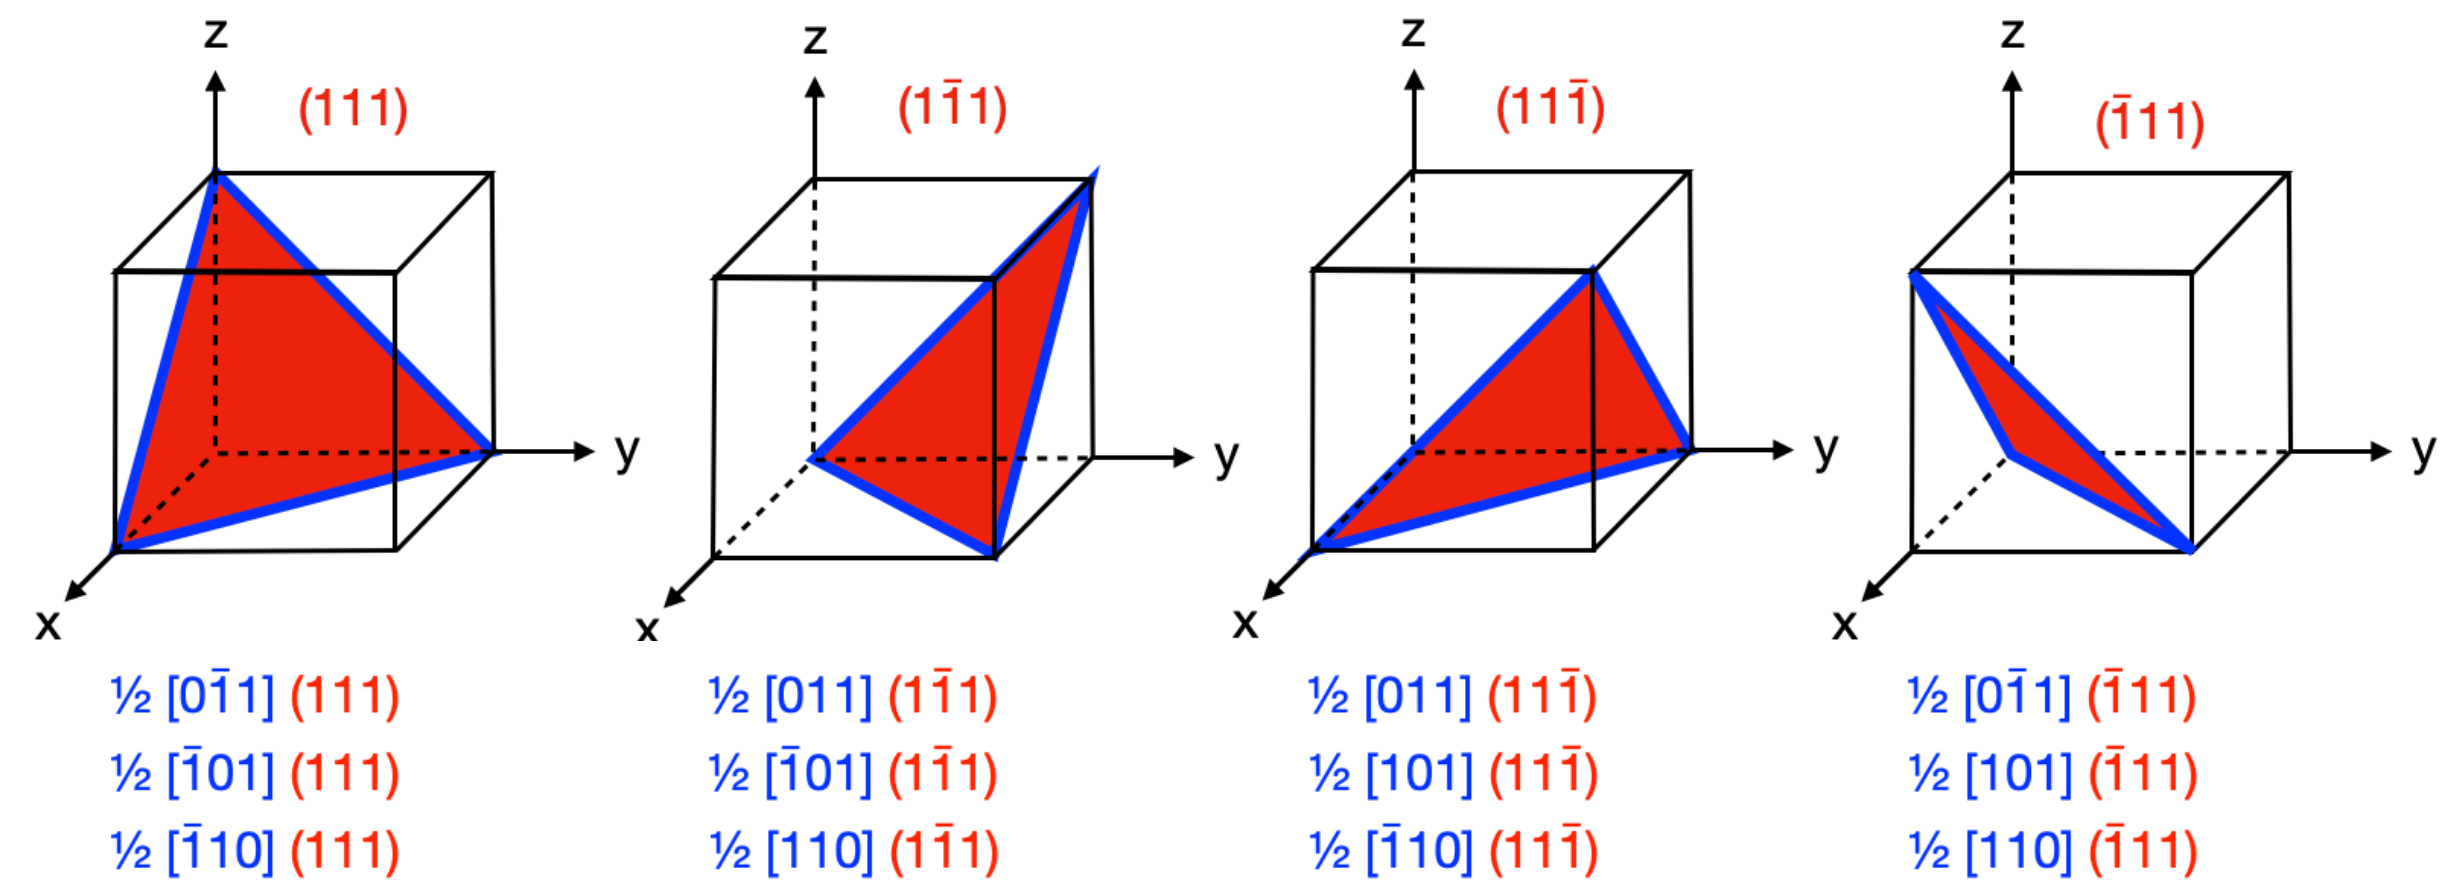
\includegraphics[width=0.8\textwidth]{media/FBB_miller.png}
\end{figure*}

\subsubsection{Slip systems in HCP metals (Miller indices)}
HCP metals are closely packed but deform on only one slip plane with 3 slip systems, resulting in limited ductility
(e.g. Ti, Zn, Mg). 
\begin{figure*}[ht!]
  \centering
  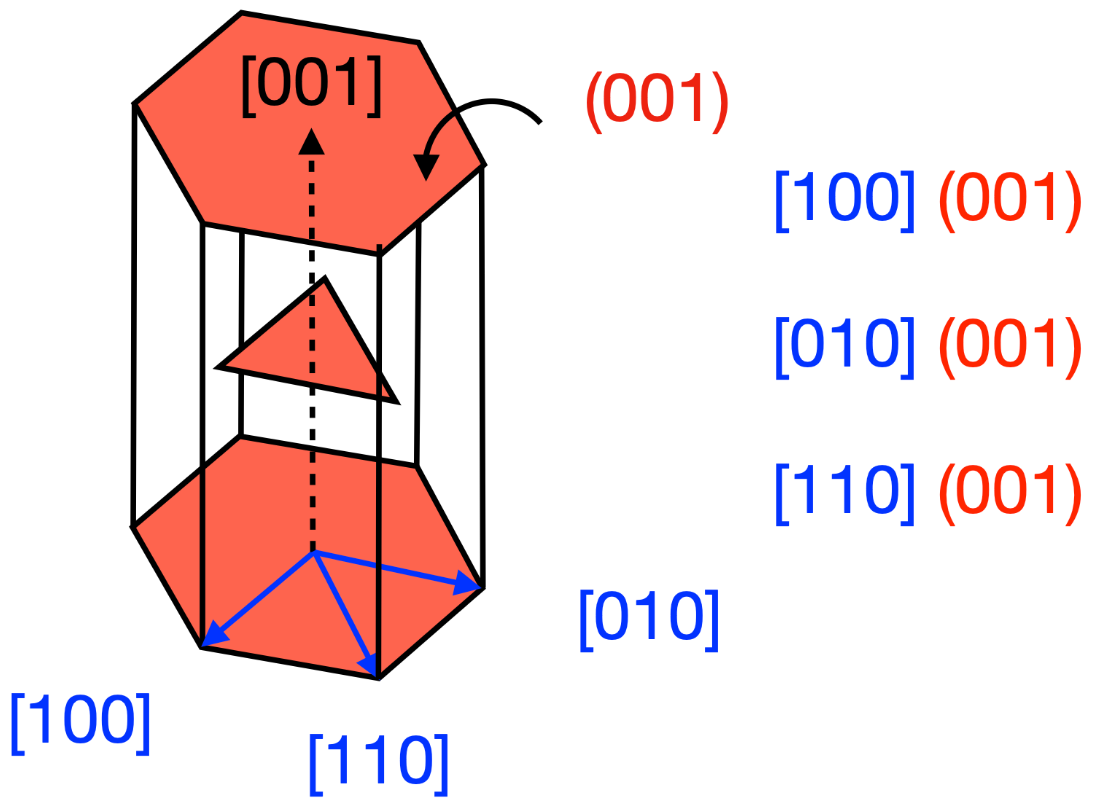
\includegraphics[width=0.35\textwidth]{media/HCP_miller.png}
\end{figure*}

\newpage
\subsubsection{Slip systems in BCC metals (Miller indices)}
BCC metals have 48 slip systems but are less closely packed, leading to higher strength
and lower ductility (e.g. $\alpha$-Fe, Cr, W, Mo, Ta, Nb)

\begin{minipage}[t]{0.6\textwidth}
  \centering
  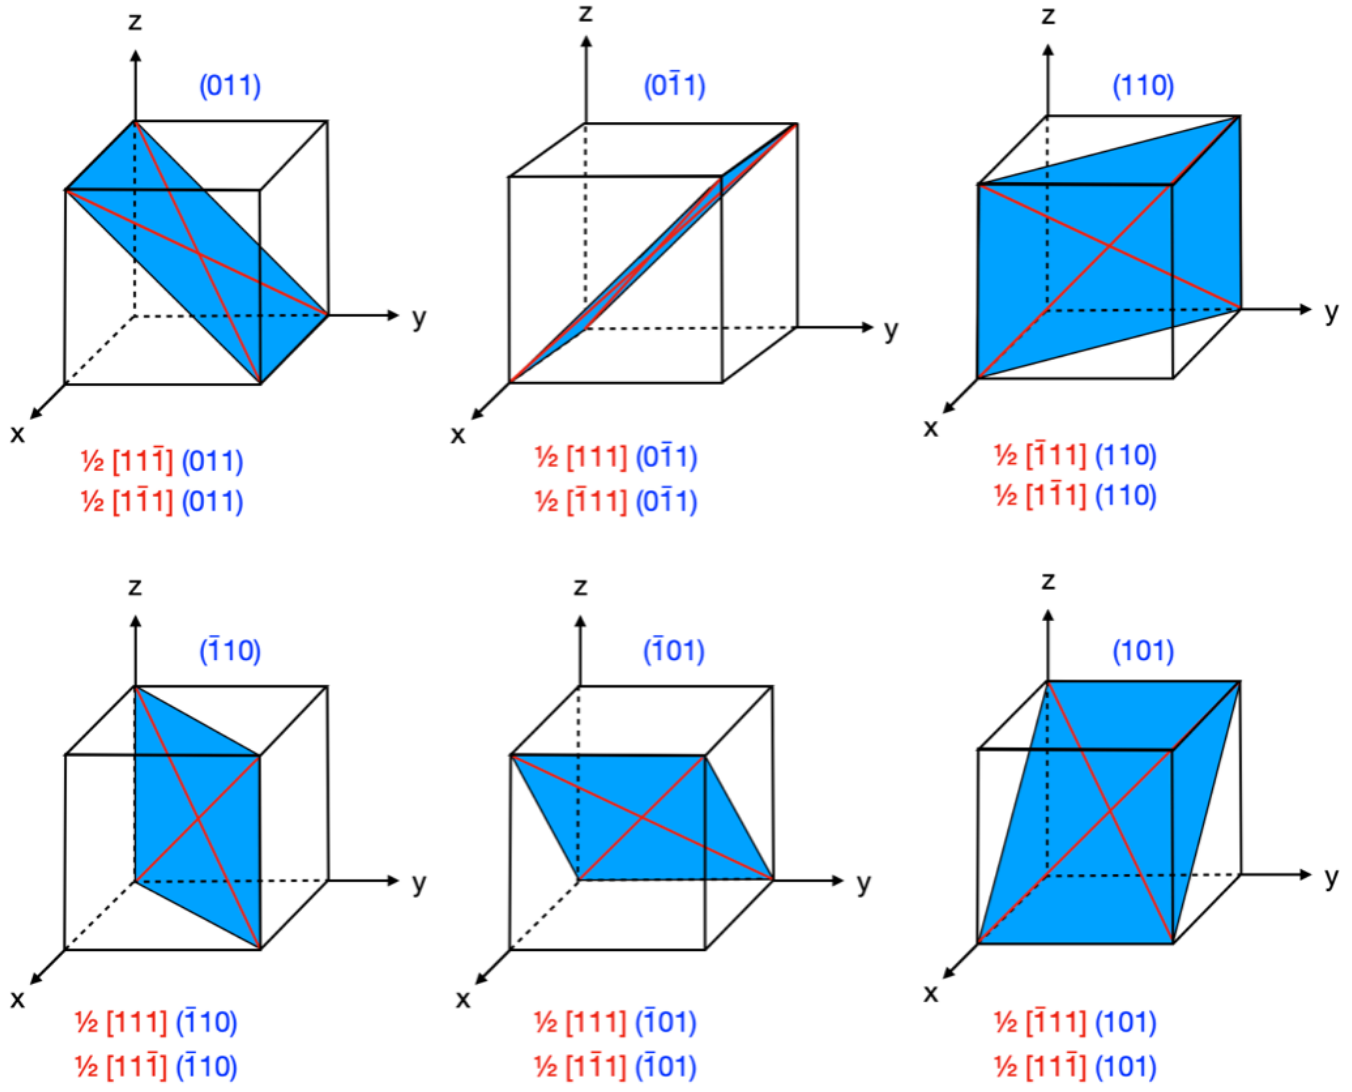
\includegraphics[width=\textwidth]{media/BCC_miller_major.png}
  \textbf{12 major slip systems:} 6 $\left\{110\right\}$ slip planes\\
  \textbf{2 slip directions:} $1/2 \langle 111 \rangle$ each
\end{minipage}
\begin{minipage}[t]{0.4\textwidth}
  \centering
  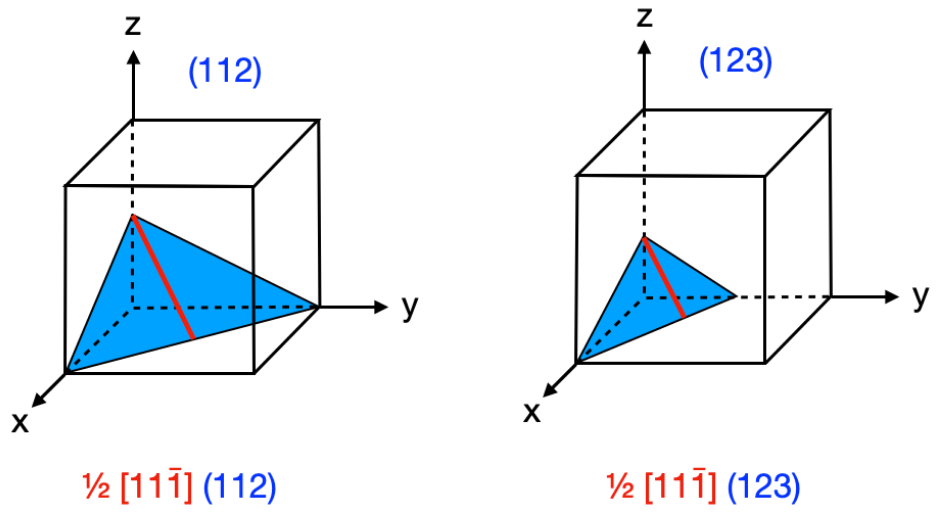
\includegraphics[width=\textwidth]{media/BCC_miller_minor.png}
  \textbf{36 minor slip systems:}\\
  12x $1/2 \langle111\rangle \left\{112\right\}$

  24x $1/2 \langle111\rangle \left\{123\right\}$
\end{minipage}

\begin{wrapfigure}{r}{0.2\textwidth}
  \centering
  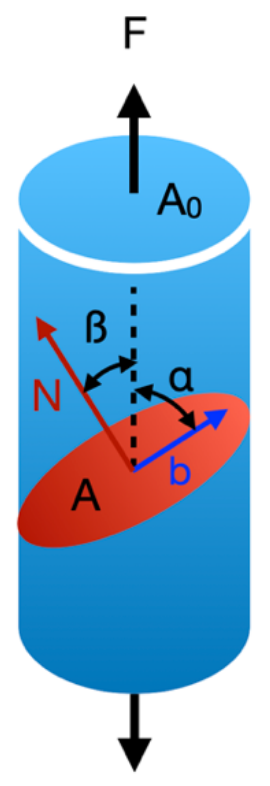
\includegraphics[width=0.5\linewidth]{media/schmids_law.png}
\end{wrapfigure}

\phantom{}

\subsection{Schmid's law of critical resolved shear stress}
The Schmid's law states that slip begins in a crystalline material when the resolved shear
stress on a slip system reaches a critical value.
\begin{itemize}
  \item PLastic deformation occurs only on closely packed slip planes where the applied
    shear stress exceeds a critical value
  \item Under uniaxial loading, the maximum shear stress acts on slip planes inclined
    at 45$^\circ$ to the load axis
\end{itemize}
\wrapfill

\vspace*{-3cm}

\subsection{Correlation between metals crystal structure and ductility}

\renewcommand{\arraystretch}{1.3} % spacing
\begin{tabularx}{\textwidth}{|c|X|l|X|X|}
\hline
\textbf{Metal} & \textbf{Ductility} & \textbf{Packing structure} & \textbf{Slip systems} & \textbf{Slip system orientation} \\
\hline
\textbf{FCC} &
Highest ductility among metals &
Closest-packed (74\%) &
4 slip planes $\rightarrow$ 12 slip systems &
Very high probability of favorable orientation (Schmid's law) \\
\hline
\textbf{BCC} &
Lower ductility than FCC, but still generally good &
Less closely packed (68\%) &
Many slip planes and slip systems &
Strength often higher than FCC metals \\
\hline
\textbf{HCP} &
Limited ductility under normal conditions &
Closest-packed (74\%) &
Only 1 slip plane $\rightarrow$ 3 slip systems &
Low probability of favorable orientation ($-45^\circ$ to load axis) \\
\hline
\end{tabularx}

\newpage
\subsection{Particulatiries in BCC metals}
\subsubsection{Cottrell atmospheres and Dislocation pinning}
\begin{itemize}
  \item In $\alpha-$iron with a BCC structure (ferrite), the octahedral sites for interstitial atoms such as carbon or nitrogen are much smaller than in $\gamma-$iron with an FCC structure (austenite)
  \item As a result, carbon atoms in ferrite preferentially diffuse into the distortion fields near dislocation lines, where more space is available, forming so-called \textbf{Cottrell atmospheres}
  \item {\color{red}These atmospheres are responsible for the pronounced upper yield point (R$_\text{eH}$) observed in tensile tests of many BCC metals, as well as for the brittle fracture behavior at low temperature in impact tests}
  \item During plastic deformation, dislocations must first break free from the Cottrell atmosphere. This process is especially difficult at low temperatures or high strain rates, leading to strong dislocation pinning
\end{itemize}

\begin{figure*}[ht!]
  \centering
  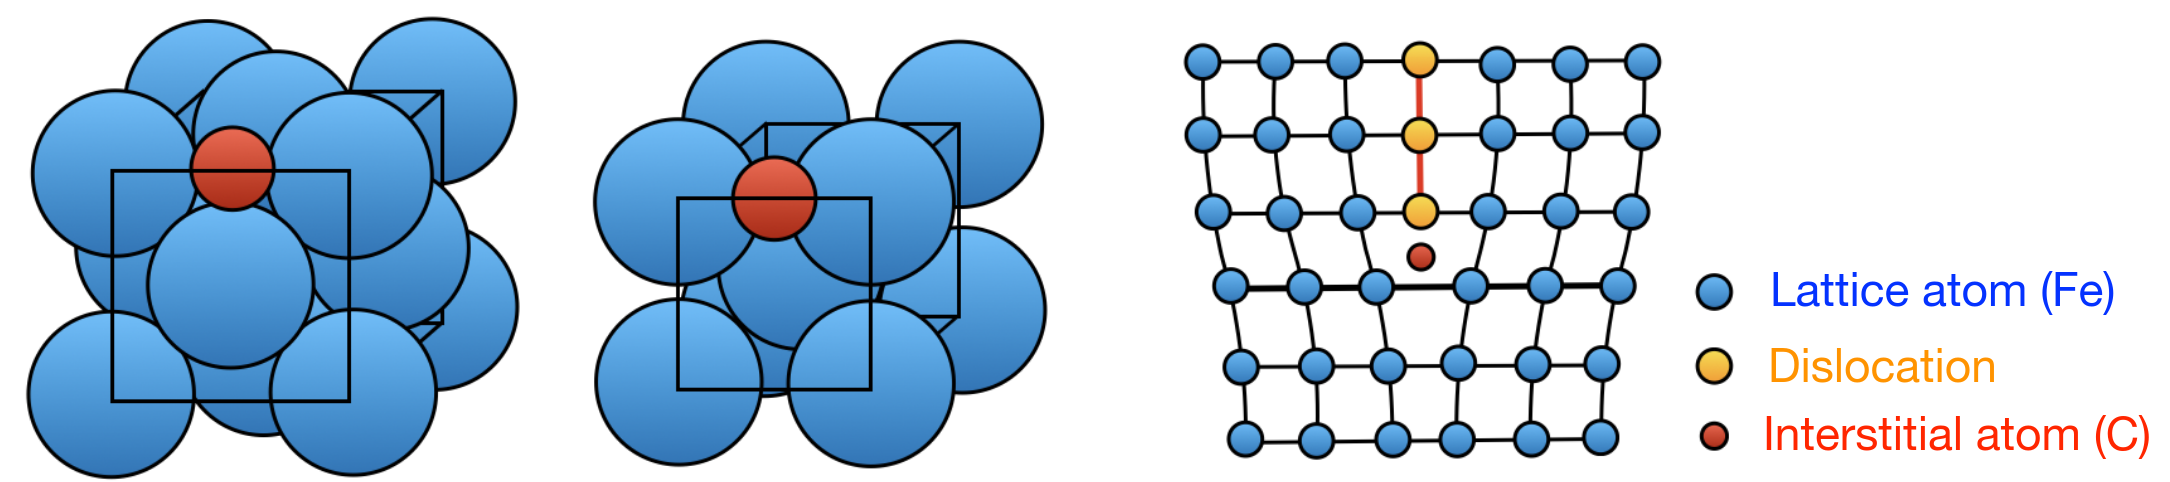
\includegraphics[width=0.8\textwidth]{media/cottrell_atmospheres.png}
  \caption*\\\vspace*{-0.25cm}{Carbon atoms occupy small octahedral sites (left), preferentially diffuse to dislocation regions (center), which forms Cottrell atmospheres that pin dislocations (right)}
\end{figure*}

\section{Strengthening mechanisms}
\subsubsection{Metals mechanisms}
Lattice defects act as deliberate obstacles that impede the motion of dislocations.

\begin{tabularx}{\textwidth}{|c|p{6.5cm}|X|p{3cm}|}
\hline \textbf{Dim} & \textbf{Lattice Defect} & \textbf{Strengthening Mechanism} & \textbf{Increase in 0.2\% Yield Strength} \\
\hline 0-D & \textbf{Substitution / Interstitial atoms} with concentration of $c$ in the solid solution crystal & Solid solution hardening & $\Delta \mathrm{R}_{\mathrm{p} 0.2} \sim \mathrm{c}^{1 / 2}$ \\
\hline 1-D & \textbf{Dislocations} (dislocation density $N$) & Strain (cold-work) hardening & $\Delta \mathrm{R}_{\mathrm{p} 0.2} \sim \mathrm{~N}^{1 / 2}$ \\
\hline 2-D & \textbf{Grain boundaries} defining an average grain size of $d$ & Grain boundary hardening\hfill {\color{red}strength and ductility still good} & $\Delta \mathrm{R}_{\mathrm{p} 0.2} \sim \mathrm{~d}^{-1 / 2}$ \\
\hline 3-D & \textbf Coherent \textbf{precepitates} with a size of $D$ (also: semi-coherent and incoherent precipitates and dispersion particles) & Precipitation hardening & $\Delta \mathrm{R}_{\mathrm{p} 0.2} \sim \mathrm{D}^{1 / 2}$ \\
\hline
\end{tabularx}

\subsubsection{0-dimensional: Solid-solution hardening}
\begin{itemize}
  \item Impurity atoms in a solid solution create lattice distortion fields that impede dislocation motion
  \item Interstitial atmos cause stronger lattice distortions than substitutional atoms, leading to a greater strengthening effect
  \item A larger atomic radius mismatch and higher impurity concentration both increase the strengthening effect
  \item \textbf{Result}: increased strength but reduced ductility
\end{itemize}

\begin{figure*}[ht!]
  \centering
  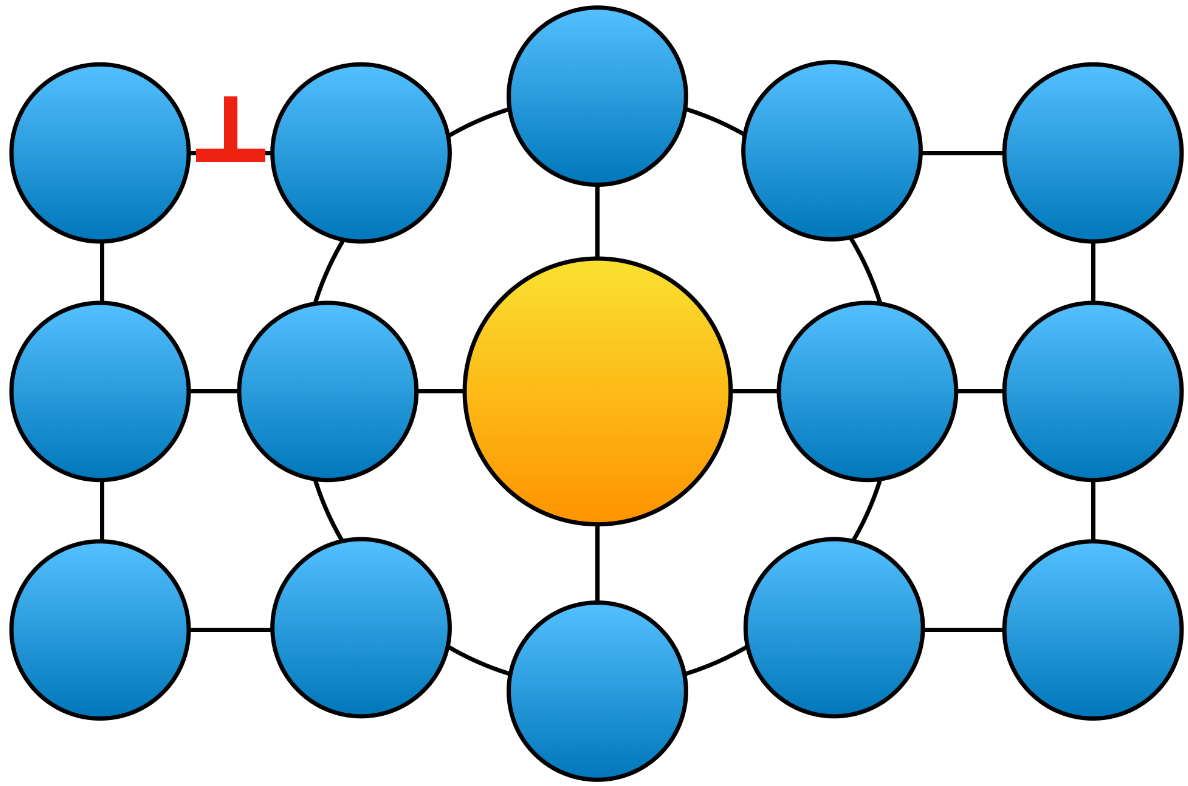
\includegraphics[width=.4\textwidth]{media/0d_strength.png}
  \caption*{Edge dislocation in a crystal lattice with a substitutional impurity atom}
\end{figure*}

\newpage
SSH application fields:
\begin{itemize}
  \item Al-Mn and Al-Mg alloys (5000 and 3000) for:
  \begin{itemize}
    \item Automotive sheet metal
    \item Airplane outer skin
    \item Beverage cans
    \item Sandwich honeycomb structures in lightweight structures
  \end{itemize}
  \item Structural and stainless steels
  \item Gold jewerly (Au with Ag, Cu, Ni, Pt, Pd, \dots)
\end{itemize}

\section{\color{red}TODO}

\newpage
\part{Strength and Ductility}
\section{Properties of material}
\begin{table*}[h!]
  \centering
  \begin{tabular}{|c|p{5cm}|p{7cm}|}
    \hline
    \textbf{Property} & \textbf{Context} & \textbf{Characteristic values}\\
    \hline
    Mechanical & Withstanding static or dynamic loads/forces/stress & Young's modulus, static strength, hardness, fatigue strength, creep strength, toughness, ductility\\
    \hline
    Technological & Material processing & Formability, welding suitability, castability, hardenability\\
    \hline
    Physical & Various functional properties & Electrical and thermal conductivity, transparency, magnetizability, refraction index, \ldots\\
    \hline
    Chemical & Resistance to normal or harsh environments & Resistance against corrsion, UV light or oxidizing agents, food safety, biocompatibility, toxicity\\
    \hline
  \end{tabular}
\end{table*}

\subsection{Failure hypotesis and Material testing methods (examples)}
\begin{table*}[h!]
  \centering
  \begin{tabular}{|p{7cm}|l|}
    \hline
    \textbf{Failure hypothesis} & \textbf{Material testing methods}\\
    \hline
    Failure of metals due the plastic deformation (dislocation slip) under static stress & Tensile test, compression test, bending test, torsion test\\
    \hline
    Failure due the crack formation and crack growth under dynamic oscillating stress & Fatigue tests (HCG, LCF)\\
    \hline
    Failure due the crack growth under sudden impact (crack growth under constant load) & Impact notch toughness test (Fractures mechanics)\\
    \hline
    Failure due the plastic deformation at high temperatures (diffusion, especially along the grain boundaries) under static stress & Creep test (or relaxation test)\\
    \hline
  \end{tabular}
\end{table*}


\section{Tensile test}
\subsection{Engineering Stress and Stress conditions}
\subsubsection{Engineering stress $\sigma$}
Engineering stress is the force $F$ acting on the original cross-sectional
area $S_0$:
\figbox{$\dm \sigma = \frac{F}{S_0}$}

\subsubsection{Normal stress}
The normal stress, similar to $\sigma$, is the force $F_N$ that acts
perpendicularly to $S_0$:
\figbox{$\dm \sigma = \frac{F_N}{S_0}$}

\newpage
\subsubsection{Shear stress}
Shear stress is the force $F_Q$ parallel to the original surface $S_0$:
\figbox{$\dm \tau = \frac{F_Q}{S_0}$}

\subsubsection{Engineering strain $\varepsilon$}
Engineering strain is the ratio of the change in length to the
original length of a material under load:
\figbox{$\dm \varepsilon = \frac{\Delta L}{L_0} = \frac{L_1 - L_0}{L_0}$}

\subsubsection{Hooke's law}
Within the elastic limit of a material, the deformation (strain) is directly proportional
to the applied stress:
\figbox{$\dm \sigma = E\cdot \varepsilon$}

\begin{figure*}[ht!]
  \centering
  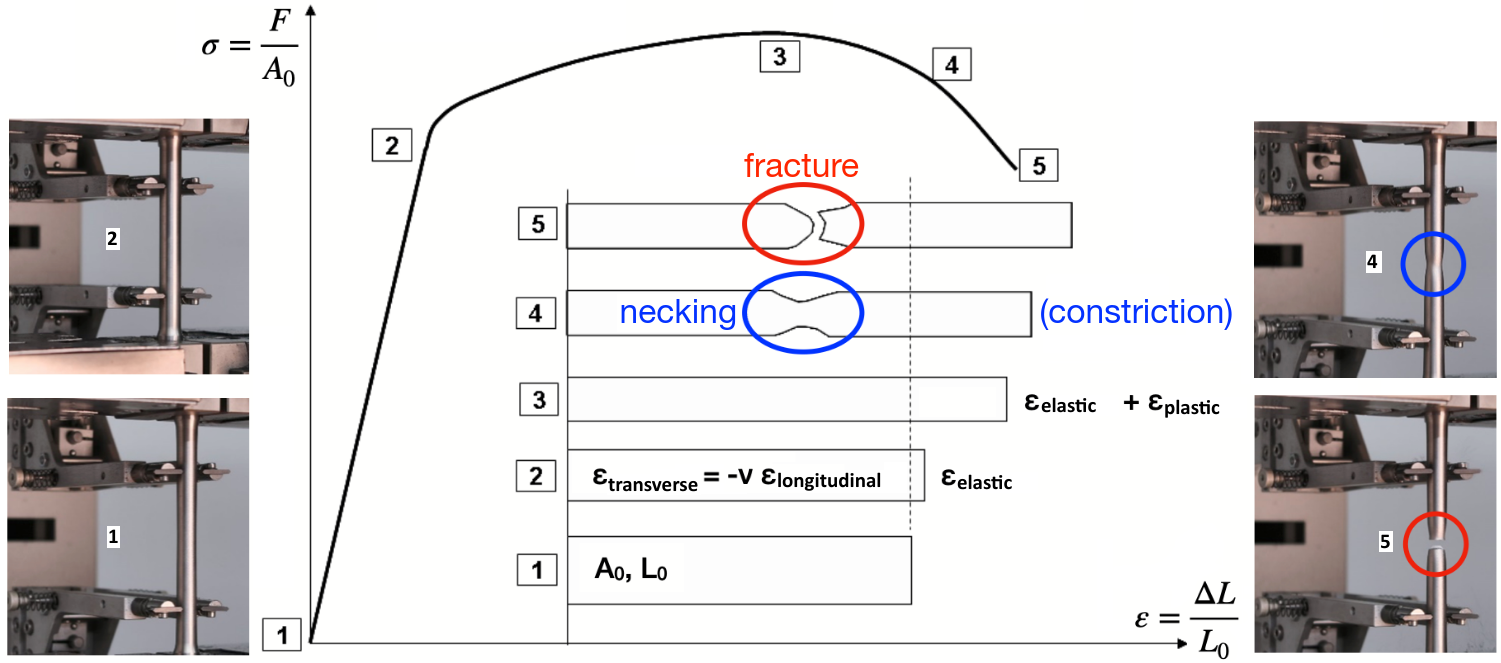
\includegraphics[width=\textwidth]{media/tensile_test.png}
  \caption*{Tensile test with of a BCC metal without the upper yield point R$_\text{eH}$}
\end{figure*}

\subsection{Elastic characteristics of some metals}
\begin{table*}[h!]
  \centering
  \begin{tabular}{|c|c|c|c|}
    \hline
    Metal & Poisson's ratio $\nu$ & Young's modulus $E$ [N/mm$^2$] & Shear modulus $G$ [N/mm$^2$]\\
    \hline
    Mg & 0.28 & 44'300 & 17'200\\
    \hline
    Al & 0.34 & 70'600 & 26'500\\
    \hline
    Ti & 0.36 & 111'800 & 40'200\\
    \hline
    $\alpha-$Fe & 0.25 & 206'000 & 82'400\\
    \hline
    Steel & 0.28 & 206'000 & 80'440\\
    \hline
    Cu & 0.35 & 122'530 & 45'130\\
    \hline
    Brass & 0.41 & 103'000 & 36'490\\
    \hline
    Zn & 0.25 & 130'010 & 41'200\\
    \hline
  \end{tabular}
\end{table*}

\newpage
\subsection{Typical stress-strain behavior of metals}
If the applied force is too big:
\begin{itemize}
  \item Starting of Dislocation slip
  \item Plastic deformation
\end{itemize}

\subsubsection{Yield Strength}
\begin{itemize}
  \item Upper Yield point R$_\text{eH}$: ferritic structural steels (BCC)
  \item 0.2\% Yield Stress R$_{\text{p}0.2}$: most other metals and alloy
\end{itemize}

\subsubsection{Graphical representation}
\begin{figure*}[ht!]
  \centering
  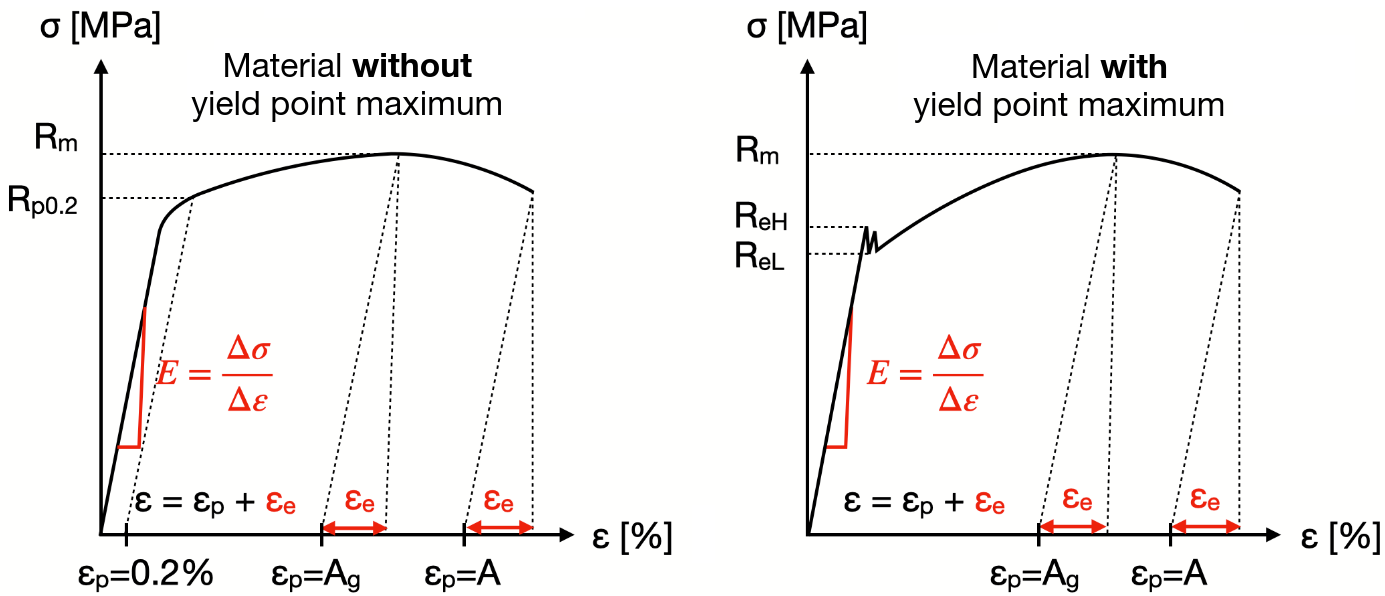
\includegraphics[width=\textwidth]{media/stress-strain_behavior.png}
\end{figure*}
\begin{minipage}[t]{.5\textwidth}
  \centering
  Without the maximum yield point:
  \begin{itemize}
    \item $\sigma_{\max} =$ R$_{\text{p0.2}}$ (0.2\% yield stress)
  \end{itemize}
\end{minipage}%
\hfill
\begin{minipage}[t]{.5\textwidth}
  \centering
  With the maximum yield point:
  \begin{itemize}
    \item $\sigma_{\max} =$ R$_{\text{m}}$
    \item Upper yield point R$_\text{eH}$
  \end{itemize}
\end{minipage}

\subsection{Young's modulus and Characteristic Strength Values}
\subsubsection{Young's modulus $E$}
The Young's modulus $E$ is measured as the slope in the linear-elastic range:
\figbox{$\dm E = \frac{\Delta \sigma}{\Delta \varepsilon}$ in [N/mm$^2$ ; (MPa)] or [kN/mm$^2$ ; (GPa)]}

\subsubsection{Yield stress $R$}
Yield stress $R$ is the stress, expressed in MPa, at which plastic deformation begins:
\begin{itemize}
  \item 0.2\% Yield stress $R_{\text{p}0.2}$ corresponds to the stress at a plastic strain of $\varepsilon_\mathrm{p} = 0.2\%$
  \item Upper yield point R$_\text{eH}$ corresponds to the maximum stress observed at the onset of yielding, mainly in ferritic structural steels
\end{itemize} 

\subsubsection{Tensile strength R$_\text{m}$}
It corresponds to the stress at the maximum of the stress-strain curve

\newpage
\subsubsection{Graphical representation}
\begin{figure*}[ht!]
  \centering
  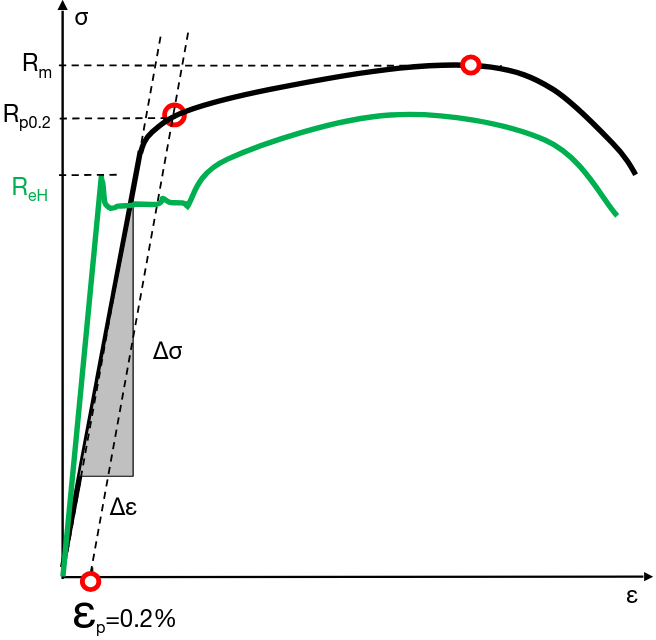
\includegraphics[width=.5\textwidth]{media/stress-strain_graph.png}
  \caption*{Note: representation not scaled; the elastic region is drawn much too flat}
\end{figure*}

\subsection{Characteristic Ductility values}
\subsubsection{Fracture Strain $A$}
Plastic strain at fracture is defined with respect to the initial specimen length $L_0$
(e.g.: $ L_0 = 50$mm is reported as $A_{50\text{mm}}$)

\begin{figure*}[ht!]
  \centering
  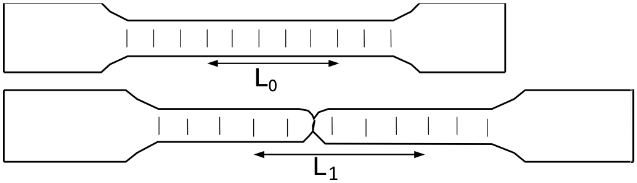
\includegraphics[width=.7\textwidth]{media/plastic_strain_at_fracture.png}
  \caption*{Plastic strain at fracture: $\dm A = \frac{L_1 - L_0}{L_0} = \varepsilon_{\text{p, fracture}}$}
\end{figure*}

\subsubsection{Uniform Strain $A_g$}
$A_g$ corresponds to the plastic strain at maximum load before necking begins.
It is very important for metal forming.

\subsubsection{Contraction at fracture $Z$}
It is the reduction of the cross-sectional area after fracture:
\figbox{$\dm Z=\frac{\Delta S}{S_0}=\frac{\left(S_1 - S_0\right)}{S_0}$}

\newpage
\begin{wrapfigure}{r}{0.4\textwidth}
  \centering
  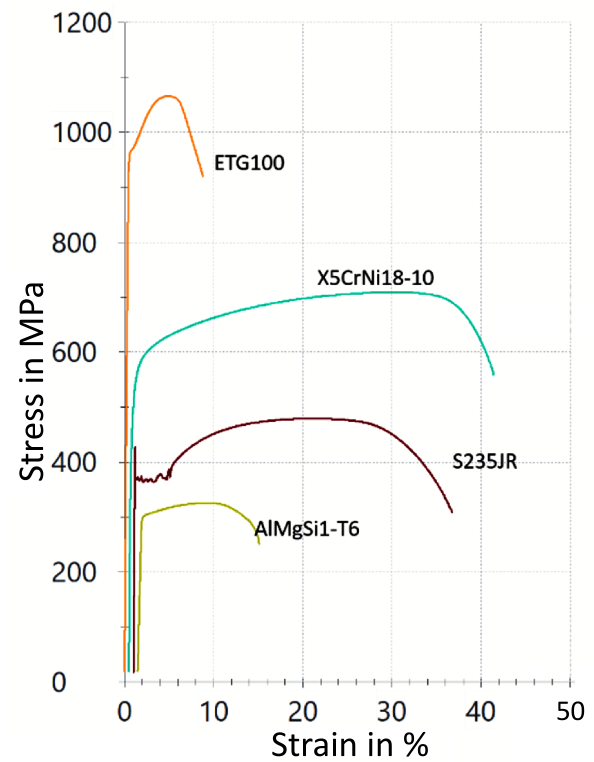
\includegraphics[width=.4\textwidth]{media/stress-strain_real-samples.png}
\end{wrapfigure}

\phantom{}

\subsection{True Stress and True Strain}
\subsubsection{True stress $\sigma*$}
True stress is the force related to the \textbf{true} cross-section
(which is constantly contracting):
\figbox{$\dm \sigma^* = \sigma\left(1+\varepsilon\right)$}

\subsubsection{Ture strain $\varepsilon*$}
True strain is the change in length relative to the \textbf{true}
length (which is constantly extending):
\figbox{$\dm \varepsilon^* = \ln\left(1+\epsilon\right)$}
\wrapfill

\vspace*{-6cm}
\subsection{Polymers Tensile test}
\begin{itemize}
  \item Characteristic values depend on test speed and temperature (0.125-500 mm/min).
  \item Creep occurs already at room temperature: creep tests and isochronus stress-strain diagrams are really relevant
  \item At high temperature and low strain rate: strength values and Young's modulus decrease, while characteristic strain values increase
  \item Characteristic values differ from materials:
  \begin{itemize}
    \item Secant modulus $E$ (determinated between $\varepsilon =$ 0.05\% and 0.25\%)
    \item Yield stress $\sigma_y$ and yield strain $\varepsilon_y$
    \item Fracture stress $\sigma_b$ and fracture strain $\varepsilon_b$
  \end{itemize}
\end{itemize}

\subsection{Summary of tensile test}
\begin{itemize}
  \item Stress-strain behavior is determined on a specimen (rod, round, flat). Standard: DIN EN EN ISO 6892
  \item Force and elongation are measured and converted into stress $\sigma$ and strain $\varepsilon$
  \item The resistance of a material to plastic deformation or fracture is referred to as its \textbf{strength}
\end{itemize}

From the stress-strain curve, the following characteristic values can be identified:
\subsubsection{Characteristic stress values}
\begin{itemize}
  \item 0.2\% Yield Strength R$_\text{p0.2}$ (for ferritic structural steels: Upper Yield Point $R_\text{eH}$):
    defines the onset of plastic deformation. This is the most important value for construction and design
  \item Tensile strength R$_\mathrm{m}$: characterizes the resistance to fracture
\end{itemize}

\subsubsection{Characteristic strain values}
\begin{itemize}
  \item Fracture strain $A$
  \item Uniform strain $A_g$
  \item Contraction at fracture $Z$
  \item $r-$ and $n-$values (relevant in metal forming) 
\end{itemize}

\subsubsection{Elastic range}
\begin{itemize}
  \item Young's modulus $E$ (Hooke's law, elastic slope)
  \item Poisson's ratio $\nu$
\end{itemize}

\newpage
\section{Other quasi-static mechanical tests}
\subsection{Bending test}
\subsubsection{Flexural strength (bend strength) $\sigma_b$}
The bend strength is the peripheral edge stress $\sigma_b$ in the
fracture point:
\figbox{$\dm \sigma_b = \frac{3FL}{2bh^2} = \frac{3F(L-L_1)}{2bh^2}$}

The Young's modulus $E$ is then calculated as:
\figbox{$\dm E = \frac{L^3\cdot F}{4bh^3\cdot f}$}

\begin{figure*}[ht!]
  \centering
  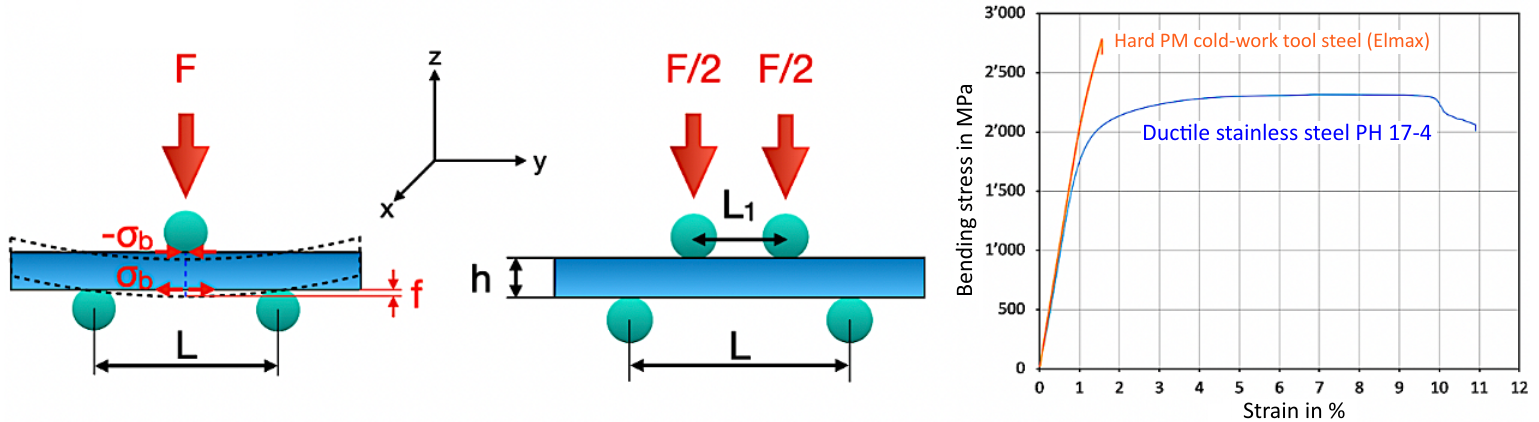
\includegraphics[width=\textwidth]{media/bending-test.png}
\end{figure*}

\subsection{Torsion test}
\begin{itemize}
  \item Less significant than tensile or bending tests
  \item Peripheral edge shear stress $\tau_R$ at fracture = torsion strength $\tau_{R, B}$
  \item A plastic shear strain at the peripheral edge of 0.4\% corresponds to a plastic strain of 0.2\% in tensile tests
  \item The 0.4\% torsion strength $\tau_{R,0.4} > R_\text{p0.2}$ from tensile tests 
  \item \fbox{$\tau_{R,0.4} \simeq 0.58\cdot R_\text{p0.2}$}
\end{itemize}

\begin{figure*}[ht!]
  \centering
  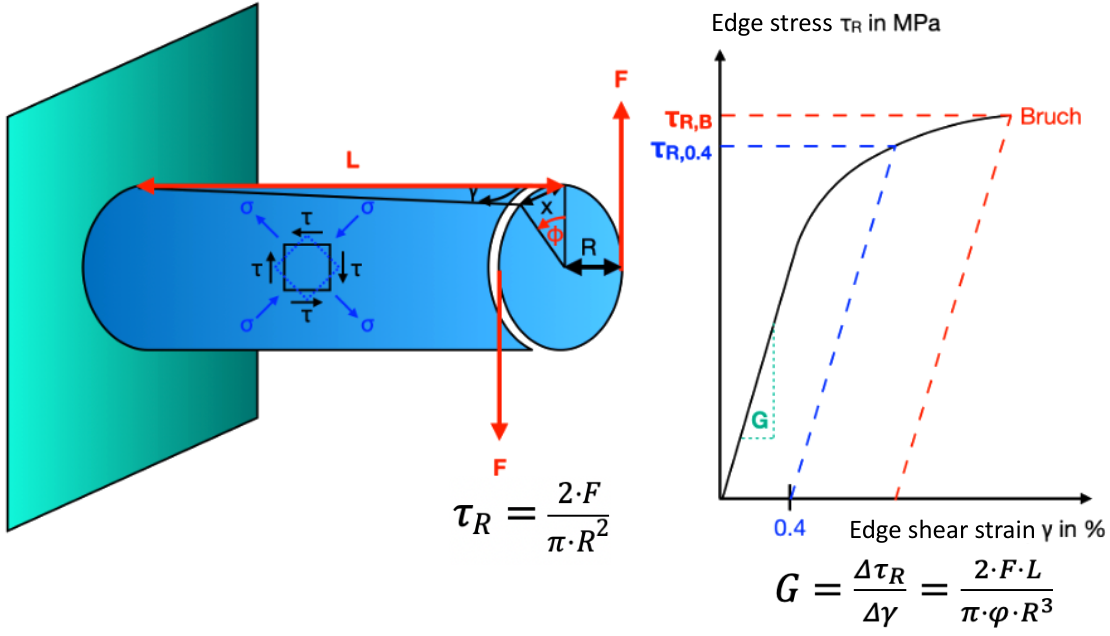
\includegraphics[width=.7\textwidth]{media/torsion-test.png}
\end{figure*}

\newpage
\subsection{Creep and Relaxation Tests (High temperatures)}
\begin{itemize}
  \item Creep occurs under constant stress; relaxation occurs under constant strain
  \item At room temperature, the static strength of metals is generally not time-dependent.
    Exceptions include: pure aluminum, and very strong metal such as tin and lead
  \item At elevated temperatures, strength becomes time-dependent and also influenced by test speed.
    Under constant load, strain does not remain constant but changes with load and time
  \item Materials with good creep resistance include ferritic and austenitic steels, cast steels, and nickel alloys.
    These are used above 400$^\circ$C in applications such as steam boilers, steam turbines, chemical reactors, industrial furnaces, gas turbines, and aircraft engines
  \item Creep and relaxation tests are essential for evaluating heat-resistant materials,
    alongside tensile and fatigue tests at elevated temperatures. 
\end{itemize}

\subsubsection{Creep test}
The creep test is easier to perform than the relaxation test, since it applies a constant
load and the resulting strain is easily measurable.
\begin{figure*}[ht!]
  \centering
  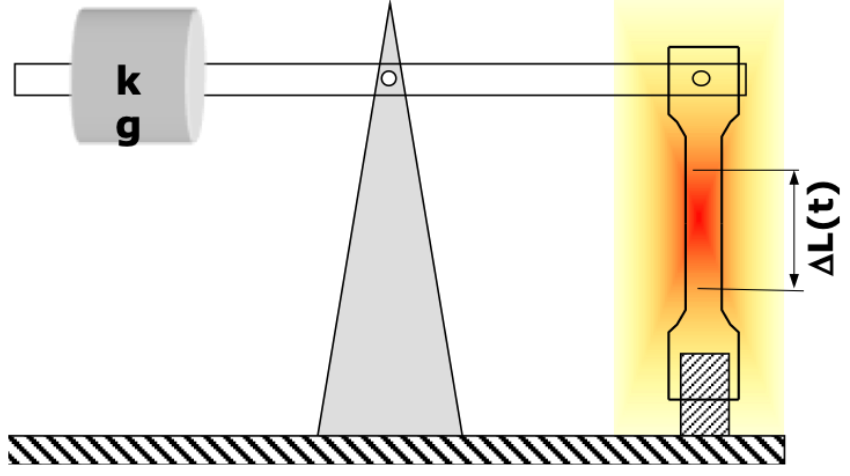
\includegraphics[width=.5\textwidth]{media/creep-test.png}
\end{figure*}

\subsection{Isochronus $\sigma-\varepsilon-$Diagram for Polymers}
\begin{itemize}
  \item In creep tests, strain increases under constant stress (for many polymers this occurs even at room temperature)
  \item Multiple creep curves can be combined into an isochronus $\sigma-\varepsilon-$diagram
  \item For different temperatures, a separate diagram is created for each temperature
\end{itemize}

\begin{figure*}[ht!]
  \centering
  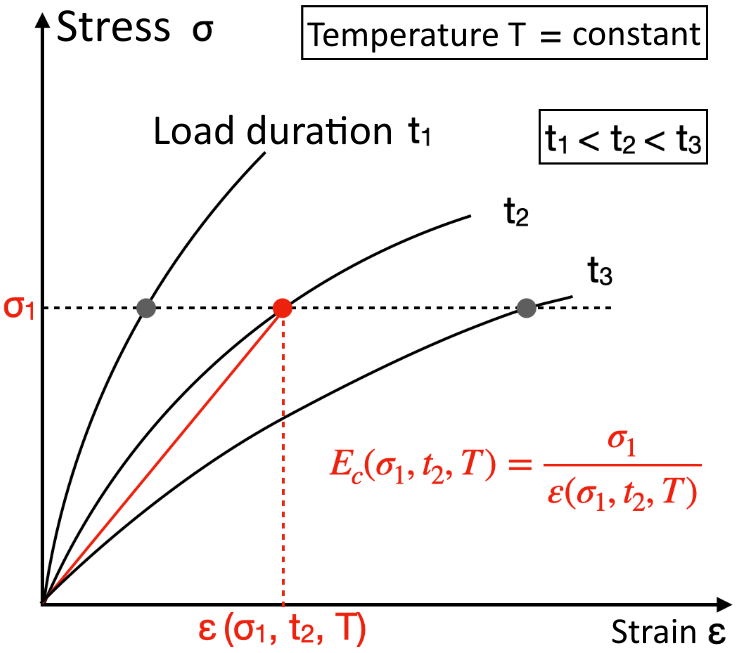
\includegraphics[width=.45\textwidth]{media/isochronus-diagram.png}
\end{figure*}

\figbox{$\dm E_c\left(\sigma, t_2, T\right) = \frac{\sigma_1}{\varepsilon\left(\sigma_1, t_2, T\right)}$}

\newpage
\part{Steel - Technology and applications}
Steel is a Carbon-iron alloy and is the most important construction material:
\begin{itemize}
  \item All Fe-C alloys with $\leq 2.1\%$ carbon (+ further alloying elements)
  \item Very good properties, adjustable over a large range:
  \begin{itemize}
    \item Strength, ductility, toughness, formability, machining, weldability
    \item Many possibilities of heat treatments (polymorphism of iron)
  \end{itemize}
  \item Innovation boost: about 75\% of all steels used today have been developed in the last 20 years
  \item China dominates steel market ($>$50\% of world production)
  \item Cost-effective (large variety of global suppliers, availability of raw materials)
\end{itemize}

\section{Steel technology}
\subsection{Blast furnace and Pig iron}
\begin{itemize}
  \item Process: reduction of iron oxide with coke \chemfig{Fe_2O_3 + 3C \to 2Fe + 3CO}
  \item Product: pig iron (3-5\% C, also contains Mn, Si, S, P)
  \item Furnace dimensions: $\sim$30m tall, $\varnothing$10-14 m
  \item Typical input/output per day:
  \begin{itemize}
    \item 16'000 t ore, 4'500 t coke, 14'000 t air
    \item \textrightarrow\ 10'000 t pig iron, 3'000 t slag, 22'000 t exhaust gas
  \end{itemize}
\end{itemize}

\begin{figure*}[ht!]
  \centering
  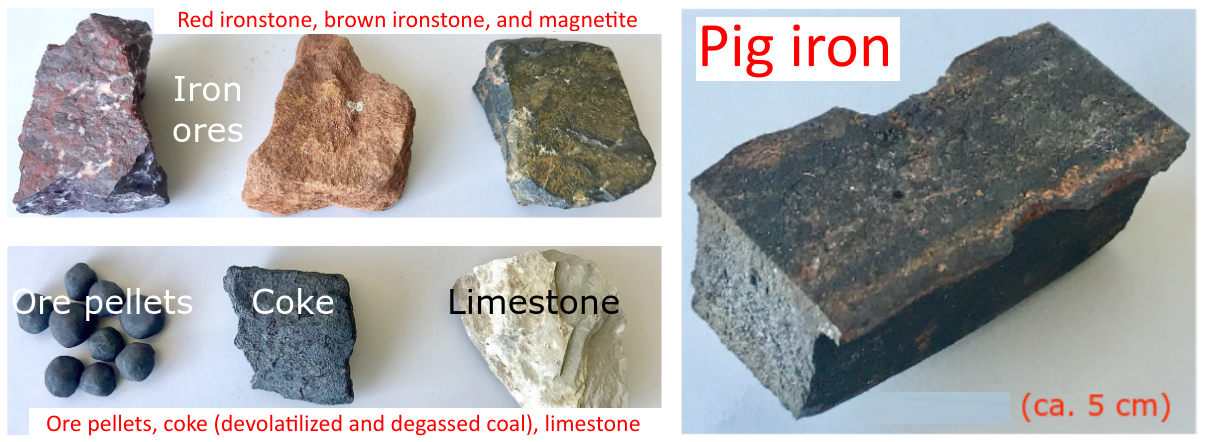
\includegraphics[width=\textwidth]{media/pig_iron.png}
\end{figure*}

\subsection{Conversion to Crude Steel}
\subsubsection{Oxygen-Blown Converter (OBC)}
\begin{itemize}
  \item Pig iron ($>$6\% C) reformed to crude steel ($<$2\% C)
  \item Pure oxygen burns off the excess carbon and other impurities
  \item Main process:
  \begin{itemize}
    \item Oxygen-blown converter (OBC, LD process)
    \item Electric furnace (EF, arc furnace, often using scrap or direct reduced iron (DRI) as input)
    \item (Historically: open-hearth furnace (OHF), now obsolete)
  \end{itemize}
  \item Continuous casting dominates ($>$30\% worldwide production)
\end{itemize}

\newpage
\begin{figure*}[ht!]
  \centering
  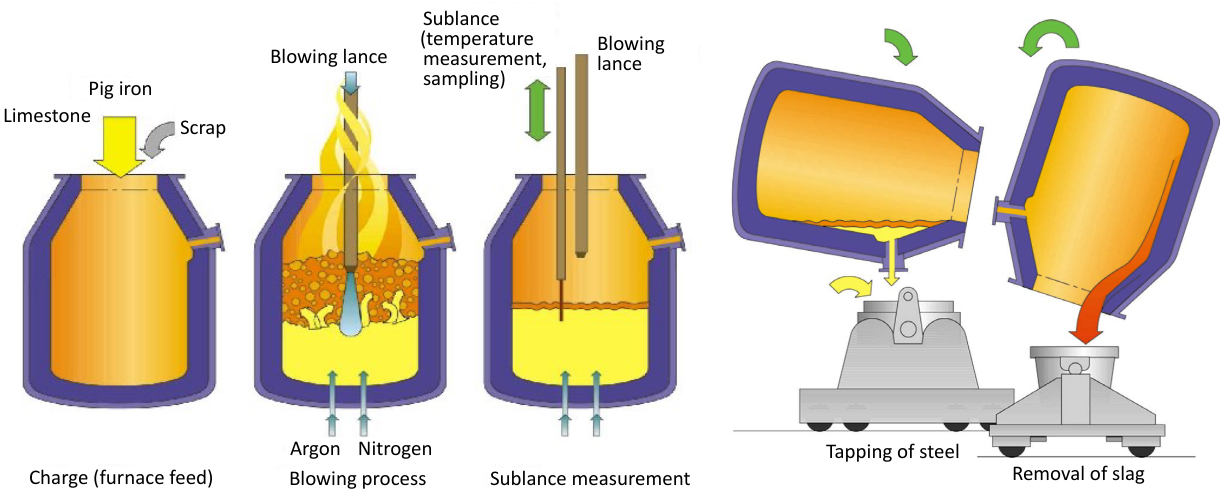
\includegraphics[width=\textwidth]{media/creation_crudesteel.png}
  \caption*{Oxygen-blown converter (OBC) process}
\end{figure*}

\subsubsection{Electric Furnace (EF)}
In Europe, about 39\% of crude steel is produced in electric furnaces (EF),
while in the World, it is about 25.8\%.

\subsection{Secondary metallurgy (Ladle metallurgy)}
\subsubsection{Purifying and alloying of the crude steel}
Procedure:
\begin{itemize}
  \item \textbf{Deoxidation}: decreasing soluble oxygen content during solidification, in order to avoid gas inclusions and splashes
  \item \textbf{Removal of impurities}: Gases and solids are rinsed out with Argon
  \item \textbf{Alloying}: Alloying wires, similar to tubes, are added to the ladle (usually via conveyor belt)
  \item \textbf{Temperature adjustment}: Casting temperature is adjusted by adding scrap or iron granules
  \item The ladle discharge is mostly continuous casting (strand casting, 88\% of the annual world production)
\end{itemize}

Special processes for archiving maximum purity:
\begin{itemize}
  \item Electroslag remelting (ESR)
  \item Vacuum arc remelting (VAR)
  \item Powder metallurgy (PM)
\end{itemize}

\begin{figure*}[ht!]
  \centering
  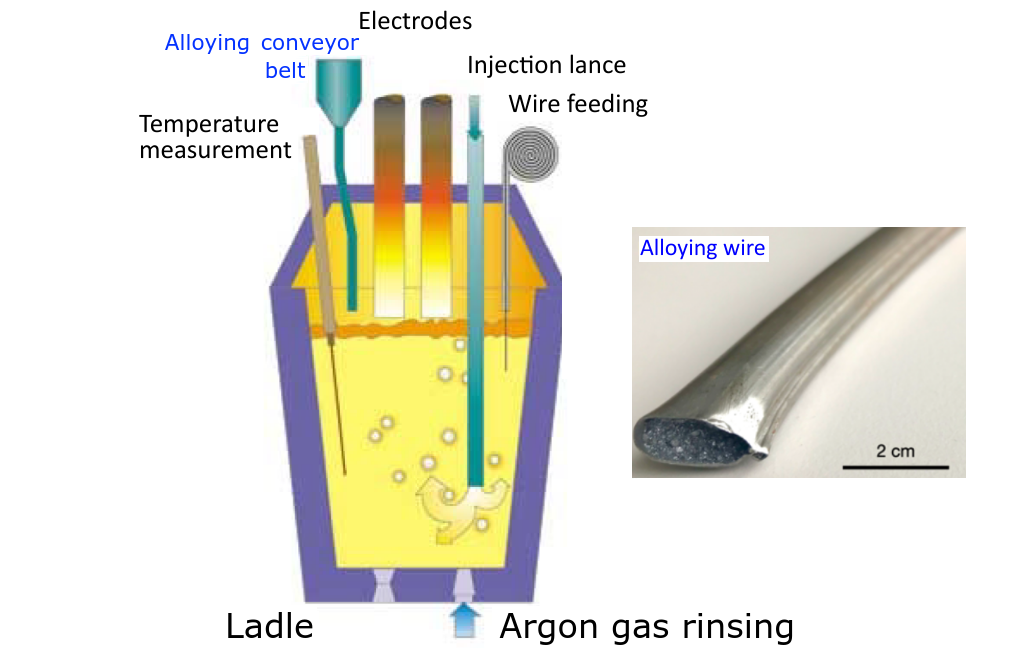
\includegraphics[width=.61\textwidth]{media/ladle_metallurgy.png}
  \caption*{Ladle metallurgy process}
\end{figure*}

\newpage
\subsubsection{Important alloying elements}
\pph{Improvement of hardenability}
The improvement of hardenability prevents the diffusion of Carbon during quenching.\\
\textbf{Most important elements:} Mn, Cr, Ni, Mo, V, Si

\pph{Fine grain}
\textbf{Al, V, Ti, Nb} in small quantities as nucleation agents (nitrides) in fine-grained structural steels.\\
\textbf{V} for grain refinement in QT steels, and \textbf{Co} for hindering grain growth in high-speed steels (HSS).

\pph{Corrosion resistance}
\textbf{Cr, Cu, Ni, Si, Mn} (all approx. $\lesssim 0.5-1\%$) to slow down the surface corrosion of steels in atmospheres and water.\\
\textbf{Cr} ($>$12\%) and \textbf{Ni} for stainless steels (e.g. AISI 304, 316).\\
\textbf{Mo} and \textbf{N} for pitting corrosion resistance in stainless steels.\\
\textbf{Ti, Nb, Ta} against intercrystalline corrosion in stainless steels after welding.

\pph{Wear and Heat resistance}
Special carbide formers: \textbf{Cr} ($>$1\%), \textbf{Mo, V}\\
Special nitride formers: \textbf{Al, V, Ti, Nb, Mo, Cr}\\

\pph{Scale resistance}
Against oxidation (scale formation), stable oxide layer against surface burn-off: \textbf{Cr, Al, Si}

\subsubsection{Resume of alloying elements functions}
\begin{table*}[h!]
  \centering
  \begin{tabular}{|l|l|}
    \hline
    \textbf{Function} & \textbf{Alloying elements}\\
    \hline
    Hardenability & Mn, Cr, Ni, Mo, V, Si\\
    \hline
    Grain refinement & Al, V, Ti, Nb\\
    \hline
    Corrosion resistance & Cr ($>$12\%), Cu, Ni, Si, Mn, Mo, N ($\lesssim$0.5-1\%)\\
    \hline
    Wear/heat resistance & Cr ($>$1\%), Mo, V, Al, Ti, Nb, Mo\\
    \hline
    Scale resistance & Cr, Al, Si\\
    \hline
  \end{tabular}
\end{table*}

\subsubsection{Electroslag remelting process (ESR)}
\pph{Principle}
\begin{itemize}
  \item Electric remelting furnace is used for refining semi-finished steel products after continuous casting
  \item Steel is remelted through a layer of \textbf{reactive slag} under alternating current (AC)
\end{itemize}

\pph{Functions of the reactive slag}
\begin{itemize}
  \item Removes impurities (e.g. P, S, O, N, H), and non-metallic inclusions
  \item Acts as refining and protective medium
\end{itemize}

\pph{Solidification}
\begin{itemize}
  \item Melt droplets pass through slag and solidify in a \textbf{water-cooled copper mold}
  \item Rapid solidification procedures:
  \begin{itemize}
    \item Fine-grained structure
    \item Homogeneously distributed carbides
  \end{itemize}
\end{itemize}

\pph{Applications}
\begin{itemize}
  \item Production of \textbf{high-purity steels} for: Toolmaking, Medical technology, Watch and precision industries, Aerospace
\end{itemize}

\pph{Alternative method}
\begin{itemize}
  \item Powder metallurgy (PM) can archieve similar levels of purity
\end{itemize}

\begin{figure*}[ht!]
  \centering
  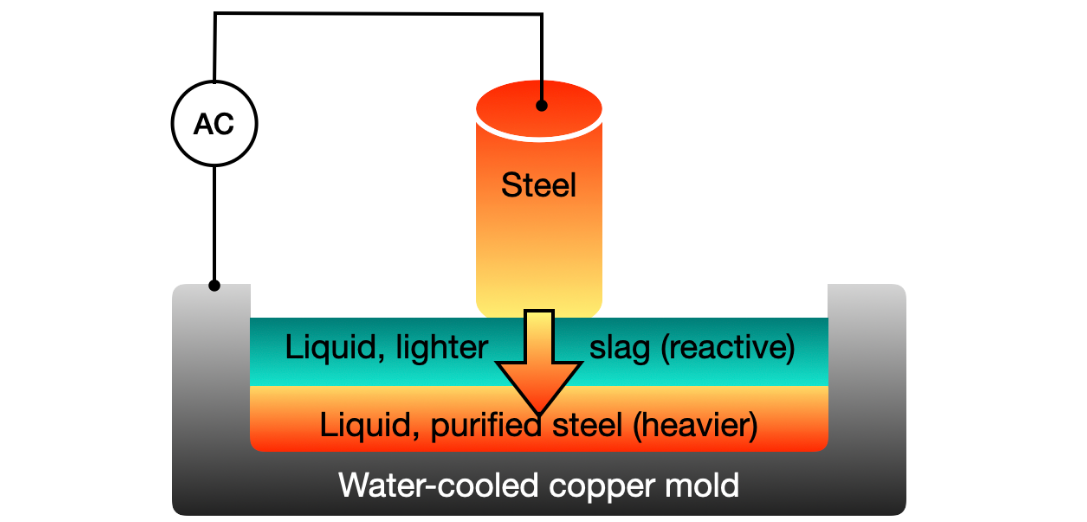
\includegraphics[width=.8\textwidth]{media/ESR.png}
  \caption*{Electroslag remelting process (ESR)}
\end{figure*}

\subsection{Continuous casting}
\begin{itemize}
  \item \textbf{Slabs}: Semi-finished product for rolling sheets (coils), foils, plates
  \item \textbf{Billets}: Semi-finished product for rolling wires, rods, profiles
  \item Wires \textrightarrow\ screws, nails, spheres, smaller rods
  \item Rods \textrightarrow\ shafts, axles, larger profiles
  \item Cold drawing \textrightarrow\ good surface quality, high precision
  \item ETG \textrightarrow\ high strength
  \item Most steel ($>$90\%) is strand-cast
\end{itemize}

\subsection{Recycling and Green Steel}
\begin{itemize}
  \item Direct hydrogen reduction instead of blast furnace \textrightarrow\ Up to 95\% lower CO$_2$ emissions, but high costs
  \item Hydrogen supply:
  \begin{itemize}
    \item H$_2$ produced by electrolysis of water
    \item Powered with renewable electricity (wind, solar)
  \end{itemize}
  \item Iron ore reduction
  \begin{itemize}
    \item Iron ore directly reduced with \textbf{green hydrogen} (DRI) to forme sponge iron
    \item By-product: \textbf{water vapor} instead of CO$_2$
  \end{itemize}
  \item Steel production
  \begin{itemize}
    \item Sponge iron charged to an \textbf{electric arc furnace} (EAF) to produce crude steel
    \item Furnace operated with green electricity
  \end{itemize}
\end{itemize}

\newpage
\subsection{Summary of Steel Technology}
\subsubsection{Blast furnace}
\begin{itemize}
  \item Iron ore reduced to \textbf{pig iron} in a blast furnace
\end{itemize}

\subsubsection{Crude steel production}
\begin{itemize}
  \item Pig iron refined to \textbf{crude steel} by reducing carbon content
  \item Oxygen-Blown Converter (\textbf{OBC}): refining with oxygen
  \item Electric Furnace (\textbf{EF}): melts scrap steel or direct-reduced iron (sponge iron) to crude steel
\end{itemize}

\subsubsection{Secondary metallurgy}
\begin{itemize}
  \item Crude steel further purified and adjusted to final composition in a ladle furnace
  \item \textbf{Processes}:
  \begin{itemize}
    \item Deoxidation (chemical or vacuum)
    \item Advanced purification (electroslag remelting (ESR), vacuum arc remelting (VAR), powder metallurgy (PM))
    \item Alloying additions
  \end{itemize}
\end{itemize}

\subsubsection{Semi-finished products}
\begin{itemize}
  \item Produced mainly by \textbf{continuous casting} (slabs, billets)
  \item Formed into sheets, plates, wires, rods, pipes, and profiles by hot or cold rolling/drawing
\end{itemize}

\section{Microstructure formation}
\subsection{Polymorphism of Iron}
\subsubsection{$\delta$-iron}
$\delta$-iron is a phase of iron with a BCC structure. It is stable above 1392$^\circ$C, and
it's not ferromagnetic. Has a limited technical relevance.

\subsubsection{$\gamma$-iron (austenite)}
$\gamma$-iron, also called austenite, is a phase of iron with a FCC structure.
It is stable between 911 - 1392$^\circ$C. It's not ferromagnetic, and is soluble up
to 2\% C, 100x more than $\alpha$-iron. Its high solubility is due to larger interstitial
sites and reduced lattice distorsion from carbon atoms.

\subsubsection{$\alpha$-iron (ferrite)}
$\alpha$-iron, also called ferrite, is a phase of iron with a BCC structure.
It's stable below 911$^\circ$C. It's not ferromagnetic between 769-911$^\circ$C, but it
becomes ferromagnetic below the \textbf{Curie temperature}, so $<$769$^\circ$C.
It has very low carbon solubility, maximum 0.02\% C.

\begin{figure*}[ht!]
  \centering
  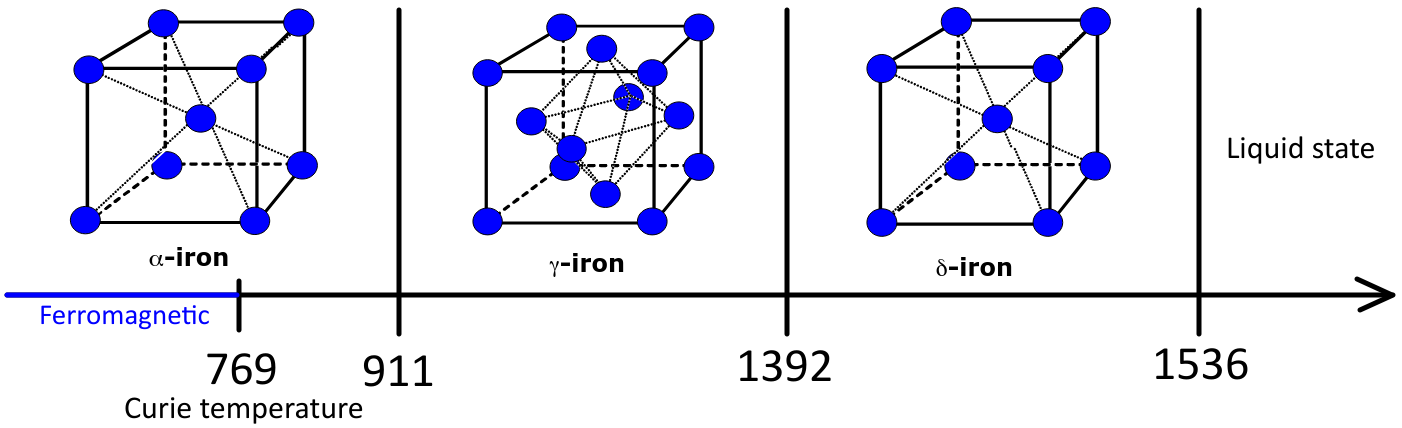
\includegraphics[width=\textwidth]{media/iron_polymorphism.png}
\end{figure*}

\newpage
\subsection{Phase transformations}
\subsubsection{Microstructure formation of Steel (Slow Cooling)}

\subsection{\color{red}TODO}
I AM JUST AT SLIDE 22 OVER 103 I ain't reading allat. gn
\begin{center}
  
\includegraphics[width=.3\textwidth]{media/bruh.png}
\end{center}

\newpage
\part{Hardness and Toughness}
\section{Hardness}
Hardness is a measure of resistance against localizer plastic deformation. It is often
considered a minimally invasive way of estimating material strength.

\subsection{Hardness testing}
\subsubsection{Common testing methods}
\begin{table*}[h!]
  \centering
  \begin{tabular}{|l|l|}
    \hline
    \textbf{Testing method} & \textbf{Application}\\
    \hline
    Vickers (HV) & Universal application\\
    \hline
    Rockwell (HRC) & Suitable for hard steels\\
    \hline
    Brinell (HB) & Used for soft steels and aluminum\\
    \hline
    Berkovich & Used in nanoindentation\\
    \hline
    Shore A and D & For rubber and plastic\\
    \hline
  \end{tabular}
\end{table*}
\vspace*{.5cm}
Approximate relation:
\figbox{$R_m \approx 3\times HB$ or $HV$}

\subsection{Examples of Hardness Testing Procedures}
\subsubsection{Indentation depth}
Hardness is measured based on how deep the indenter penetrates the material: 
\begin{itemize}
  \item Rockwell C hardness (HRC) for hard metals
  \item Shore hardness (A,D) for polymers and elastomers
\end{itemize}

\begin{figure*}[ht!]
  \centering
  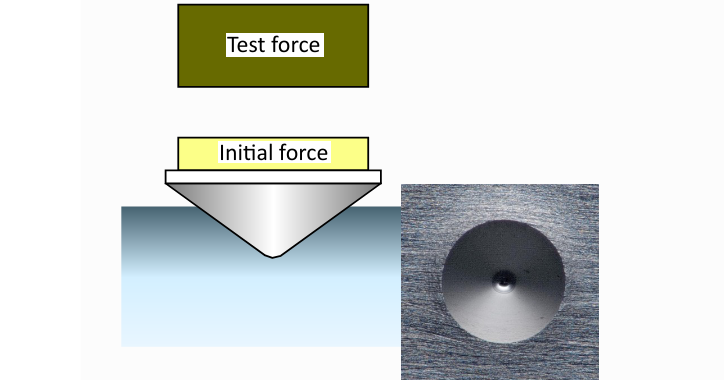
\includegraphics[width=.6\textwidth]{media/Rockwell_hardness.png}
  \caption*{Rockwell hardness testing}
\end{figure*}

\subsubsection{Indentation Area}
Hardness is determined by the surface area of the indentation left in the material:
\begin{itemize}
  \item Brinell hardness: Ball indenter for soft metals
  \item Vickers hardness: Diamond pyramind indenter, universal application
\end{itemize}

\begin{figure*}[ht!]
  \centering
  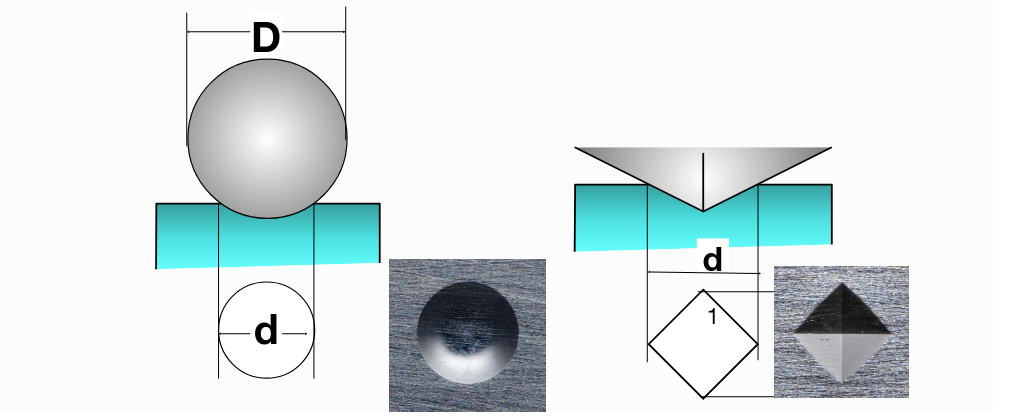
\includegraphics[width=.6\textwidth]{media/area_hardness.png}
  \caption*{Brinell hardness testing (left), Vickers hardness testing (right)}
\end{figure*}

\newpage
\subsection{Conversion of Hardness values and Tensile strength (Steels)}
Hardness v alues can be correlated to tensile strength. Conversion tables are available to
relate HV, HB, and HRC to ultimate tensile strength in MPa.

\subsubsection{Hardness - Tensile strength conversion table (Steels)}
\begin{table*}[h!]
  \centering
  \begin{tabular}{|c|c|c|c|}
    \hline
    \makecell{\textbf{Tensile strength}\\\textbf{in MPa}} &
    \makecell{\textbf{Vickers hardness}\\\textbf{HV}} &
    \makecell{\textbf{Brinell hardness}\\\textbf{HB}} &
    \makecell{\textbf{Rockwell hardness}\\\textbf{HRC}} \\
    \hline
     & 900 & & 67.0 \\
    \hline
     & 850 & & 65.6 \\
    \hline
     & 800 & & 64.0 \\
    \hline
     & 750 & & 62.2 \\
    \hline
     & 700 & & 60.1 \\
    \hline
    2180 & 650 & 618 & 57.8 \\
    \hline
    1995 & 600 & 570 & 55.2 \\
    \hline
    1810 & 550 & 523 & 52.3 \\
    \hline
    1630 & 500 & 475 & 49.1 \\
    \hline
    1455 & 450 & 428 & 45.3 \\
    \hline
    1290 & 400 & 380 & 40.8 \\
    \hline
    1125 & 350 & 333 & 35.5 \\
    \hline
    965 & 300 & 285 & 29.8 \\
    \hline
    800 & 250 & 238 & 22.2 \\
    \hline
    640 & 200 & 190 & \\
    \hline
    480 & 150 & 143 & \\
    \hline
    320 & 100 & 95 & \\
    \hline
  \end{tabular}
\end{table*}

\newpage
\section{Notch Impact Toughness}
\subsection{Impact Notch Toughness Test (Charpy)}
\begin{itemize}
  \item Applied mainly to structural steel (BCC, such as shipbuilding, bridges, oil platforms, pylons)
  \item The test determines:
  \begin{itemize}
    \item The transition temperature from ductile to brittle fracture
    \item The absorbed impact energy (``notch toughness'')
  \end{itemize}
  \item Failure hypotesis: Crack propagation under sudden, high-impact loads
\end{itemize}

\subsection{Toughness explaination}
\subsubsection{Material behavior}
\begin{itemize}
  \item \textbf{Tough material}: Absorb high energy before fracture (e.g. leather)
  \item \textbf{Brittle material}: Fracture with little energy absorption (e.g. glass)
\end{itemize}

\subsubsection{Energy criterion}
\begin{itemize}
  \item \textbf{Ductile fracture}: Defined ductile if absorbes $> 27$ J of the impact energy
  \item \textbf{Brittle fracture}: Defined brittle if absorbes $> 27$ J of the impact energy
\end{itemize}

\subsubsection{Stress State dependence}
\begin{itemize}
  \item Monoaxial (tensile test): Material can yield in lateral directions
  \item Biaxial (pressure vessels): Yield possible in one direction
  \item Triaxial (notches): No yielding possible, leads more likely to brittle failure
\end{itemize}

\subsection{Charpy Test}
The Charpy impact test evaluates a material's toughness by measuring the energy absorbed
during fracture under a sudden impact load. It is widely used to determine the
ductile-brittle transition temperature of steels and to compare the toughness of different
alloys

\subsubsection{Test setup}
\begin{itemize}
  \item Specimen: Standard rectangular bar, with a V- or U-shaped notch at the center
  \item The V- or U-notch creates a stress concentration, forcing tracture to start there
  \item Impact: A heavy pendulum strikes the specimen at the opposite side of the notch, producing fracture
  \item Measurement: The energy absorbed is read from a calibrated scale linked to the pendulum swing
\end{itemize}

\subsubsection{Differences between Charpy and Izod impact tests}
\begin{table*}[h!]
  \centering
  \begin{tabular}{|l|l|l|}
    \hline
    & \textbf{Charpy} & \textbf{Izod}\\
    \hline
    \textbf{Types of Notches} & U- and V-Notch & V-Notch only\\
    \hline
    \textbf{Specimen Position} & Horizontally & Vertically\\
    \hline
    \textbf{Material Tested} & Metals only & Plastic and metals\\
    \hline
    \textbf{Striking point} & Middle of the sample & Upper tip of the sample\\
    \hline
    \textbf{Specimen dimension} & 55x10x10 mm & 75x10x10 mm\\
    \hline
  \end{tabular}
\end{table*}

\newpage
\subsection{Fracture types}
\begin{figure*}[ht!]
  \centering
  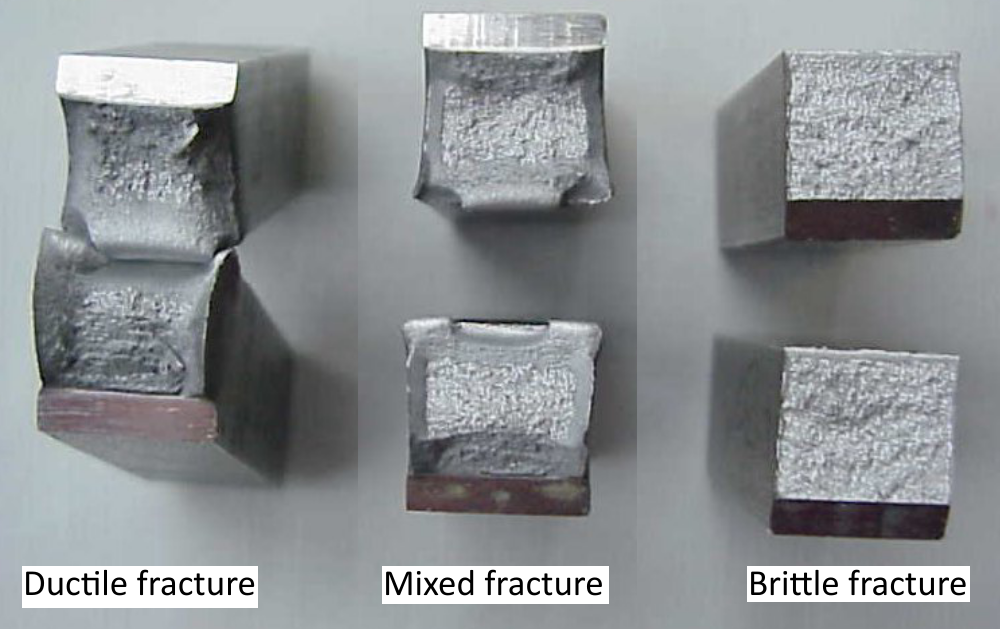
\includegraphics[width=.6\textwidth]{media/fracture_surfaces.png}
\end{figure*}

\subsection{Absorbed Energy - Temperature Graph}
\begin{figure*}[ht!]
  \centering
  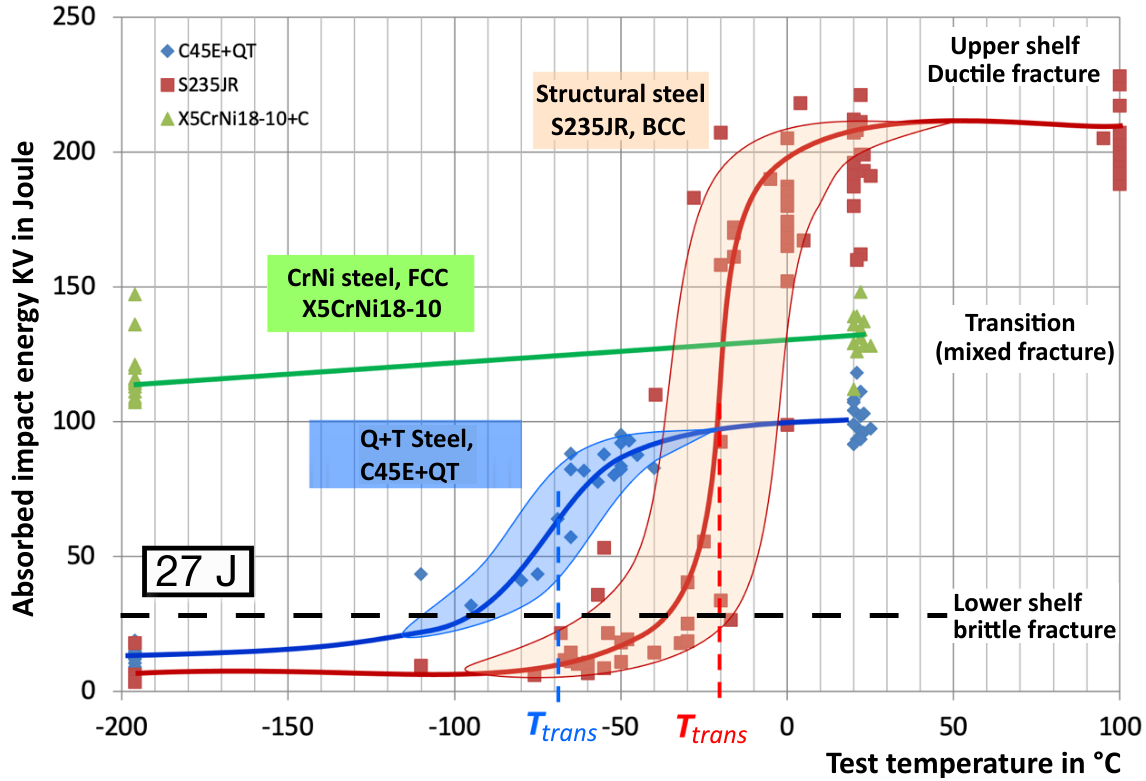
\includegraphics[width=\textwidth]{media/energy_temperature_impact_graph.png}
\end{figure*}

\subsection{BCC brittle behavior at low temperatures}
\subsubsection{Cottrell Atmospheres}
\begin{itemize}
  \item Packing efficiency: in $\alpha$-iron with BCC structure, the octahedral sites for interstitial atoms (e.g. carbon, nitrogen) are much smaller than in $\gamma$-iron with an FCC structure
  \item C solubility and diffusivity higher in BCC: small intestitial atoms, especially carbon, preferentially diffuse into the stress fields around dislocation lines, where more space is available
  \item This leads to the formation of Cottrell atmospheres, which lock dislocations by clustering interstitial atoms around them
\end{itemize}

\newpage
\subsubsection{Dislocation pinning}
\begin{itemize}
  \item Cottrell atmospheres cause a pronounced upper yield point R$_\text{eH}$ in tensile tests of many BCC metals
  \item They are also responsible for the brittle fracture behavior of BCC metals at low temperatures, as revealed by the notch impact test
  \item For plastic deformation to occur, dislocations must first break away from the Cottrell atmospheres
  \item Hardening a metal reduces its ductility, since the molecules cannot slip freely anymore, causing brittleness
  \item At low temperatures or high strain rates, this release is particularly difficult, leading to dislocation pinning and increased brittleness
\end{itemize}

\subsection{Absorbed Notch Impact Energy}
The absorbed notch impact energy indicates a material's resistance to brittle fracture and is
widely used to compare the toughness of structural steels and quenched-and-tempered (Q+T) steels:

\begin{table*}[h!]
  \centering
  \renewcommand{\arraystretch}{1.3}
  \begin{tabular}{|c|c|c|c|}
    \hline
    \makecell{\textbf{Test temperature}\\\textbf{in $^\circ$C}} &
    \makecell{\textbf{Absorbed Notch}\\\textbf{Impact Energy $\geq$ 27 J}} &
    \makecell{\textbf{Absorbed Notch}\\\textbf{Impact Energy $\geq$ 40 J}} &
    \makecell{\textbf{Absorbed Notch}\\\textbf{Impact Energy $\geq$ 60 J}}\\
    \hline
    20 & JR & KR & LR \\
    \hline
    0 & JO & KO & LO \\
    \hline
    -20 & J2 & K2 & L2 \\
    \hline
    -30 & J3 & K3 & L3 \\
    \hline
    -40 & J4 & K4 & L4 \\
    \hline
    -50 & J5 & K5 & L5 \\
    \hline
    -60 & J6 & K6 & L6 \\
    \hline
  \end{tabular}
\end{table*}

Example: S235JO \textrightarrow\ S: Steel, 235: R$_m$, JO: at 0$^\circ$C

\subsection{Summary of Notch Impact Test}
\subsubsection{Factors promoting brittle fracture}
\begin{itemize}
  \item \textbf{Notches}: Create multiaxial stress states that favor brittle failure
  \item \textbf{Sudden loading}: Allows little or no time for plastic deformation 
\end{itemize}

\subsubsection{Qualitative assessment of fracture behavior}
\begin{itemize}
  \item Differentiation between \textbf{ductile} and \textbf{brittle} failure based on absorbed impact of energy and fracture surface appearance
  \item \textbf{BCC metals}: show a clear transition from ductile failure at high temperatures to brittle failure at low temperatures
\end{itemize}

\subsubsection{Applications of the test}
\begin{itemize}
  \item Estabilishing \textbf{quality classes} and \textbf{ranking structural steels and pressure vessel steels}
  \item \textbf{Quality control} after heat treatments
\end{itemize}

\newpage
\part{Aluminum - Wrought \& Cast Alloys}
\pph{Opening exercise - Name 5 properties and 5 application of aluminum alloys}
\begin{center}
  \begin{tabular}{|c|c|}
    \hline
    \textbf{Property} & \textbf{Application}\\
    \hline
    Heat conductivity & Heat exchangers\\
    \hline
    Electrical conductivity & High voltage lines\\
    \hline
    Corrosion resistance ($<$ 10 pH only) & \makecell{Electronic appliance housing,\\ architecture}\\
    \hline
    Non-magnetic & Electronic appliance housing\\
    \hline
    Light-weight & Aerospace, automotive industry\\
    \hline
  \end{tabular}
\end{center}

\section{Introduction}
Not relevant for the exam

\subsection{Background information about aluminum}
\begin{itemize}
  \item Relatively young metal, discovered about 100 years ago
  \item More expensive than steel
  \item Density $\rho$ = 2.7 g/cm$^3$
  \item Highly malleable (FCC structure)
  \item Electrical conductivity: 37.7 S$\cdot$m/mm$^2$
  \item Young's modulus $E$: 70 GPa (lower than steel)
  \item Melting point: 660$^\circ$C (lower for cast alloys)
  \item Naturally passivated: resistant to water and weather within pH 4.5 -- 8.5
  \item Food-safe
  \item Poor corrosion resistance at pH $>$10 (alkaline environments such as dishwasher or concrete water)
  \item Oversaturated 5xxx alloys and high-strength 2xxx and 7xxx alloys are prone to corrosion
\end{itemize}

\subsection{Aluminum production}
\subsubsection{Bayer process}
\begin{itemize}
  \item Bauxite is crushed and dissolved in hot sodium hydroxide
  \item Aluminum hydroxide (Al(OH)$_3$) precipitates from the solution
  \item It is then calcinated (heated) to remove water, producing alumina (Al$_2$O$_3$)
\end{itemize}

\subsubsection{Smelting flux electrolysis (Hall-Héroult process)}
\begin{itemize}
  \item Alumina is dissolved in molten cryolite
  \item Al electric current passes through, reducing Al$^{3+}$ to liquid aluminum at the cathode and releasing O$_2$ at the carbon anode
\end{itemize}

\section{Designation of alloys and conditional designations}
\newpage
\subsection{Numerical Designation System (DIN EN 573-1)}
\begin{table}[ht!]
  \centering
  \begin{minipage}[t]{0.67\textwidth}
    \centering
    \begin{tabular}{|l|l|l|l|c|}
      \hline 
      \multicolumn{5}{|l|}{\color{blue}EN AW-: Wrought alloys} \\
      \hline 
      Nr. & \makecell[l]{Main alloying\\elements} & \thead{Strain-\\hardened} & {\color{red}\thead{Age-\\hardened}} & \thead{Type of\\hardening}\\
      \hline 
      1XXX & none, $>$99\% Al & \multirow{4}{*}{Yes (H)} & \multirow{4}{*}{No} & \multirow{4}{*}{\thead{Solid-solution hardened\\Cold-work hardened\\Fine-grain hardened}}\\ \cline{1-2}
      3XXX & Mn & & & \\ \cline{1-2}
      4XXX & Si & & & \\ \cline{1-2}
      5XXX & Mg, ($>$3\% corrosion) & & & \\ \hline
      2XXX & Cu & \multirow{4}{*}{in part} & \multirow{4}{*}{\color{red}Yes (T)} & \multirow{4}{*}{\thead{Precipitation\\hardened}} \\ \cline{1-2}
      6XXX & $\mathrm{Mg}+\mathrm{Si}$ & & & \\ \cline{1-2}
      7XXX & $\mathrm{Zn} +\mathrm{Mg}\ (+\mathrm{Cu}, \ldots)$ & & & \\ \cline{1-2}
      8XXX & others ($\mathrm{Li}, \mathrm{Sc}, \mathrm{Fe}$) & & & \\ \hline
    \end{tabular}
  \end{minipage}
  \hfill
  \begin{minipage}[t]{0.31\textwidth}
    \centering
    \begin{tabular}{|l|l|l|}
      \hline
      \multicolumn{2}{|l|}{\color{red}EN AW-: Cast alloys} \\
      \hline
      Nr. & \thead{Main alloying\\elements}\\
      \hline
      1XXX0 & $>$99\% Al\\
      \hline
      2XXX0 & Cu\\
      \hline
      \textbf{4XXX0} & \textbf{Si}\\
      \hline
      5XXX0 & Mg\\
      \hline
      7XXX0 & Zn\\
      \hline
      8XXX0 & Sn\\
      \hline
      9XXX0 & pre-alloys\\
      \hline
    \end{tabular}
  \end{minipage}
\end{table}

\subsection{Condition Designation (DIN EN 515)}
\begin{table}[ht!]
  \begin{minipage}[t]{0.58\textwidth}
    \centering
    \begin{tabular}{|c|l|}
      \hline
      \textbf{Letter} & \textbf{Meaning}\\
      \hline
      F & Without post-treatment / as fabricated (e.g. cast)\\
      \hline
      O & Annealed\\
      \hline
      H & \textbf{Strain hardenend}\\
      \hline
      T & \textbf{Thermally treated}\\
      \hline
    \end{tabular}
  \end{minipage}
  \hfill
  \begin{minipage}[t]{0.38\textwidth}
    \centering
    \begin{tabular}{|c|l|}
      \hline
      \textbf{Hxx} & \textbf{Meaning}\\
      \hline
      Hx1 & 1/8-hard\\
      \hline
      Hx2 & 1/4-hard\\
      \hline
      Hx4 & 1/2-hard\\
      \hline
      Hx6 & 3/4-hard\\
      \hline
      Hx8 & hard\\
      \hline
      Hx9 & extra hard (Hx8 + 14 MPa)\\
      \hline
    \end{tabular}    
  \end{minipage}
\end{table}

\begin{table}[ht!]
  \centering
  \begin{tabular}{|c|l|l|l|l|}
    \hline W & solution annealed & + quenched & (unstable) & \\
    \hline T1 & hot-formed & + quenched & & + naturally aged\\
    \hline T2 & hot-formed & + quenched & + cold-formed & + naturally aged\\
    \hline \textbf{T3} & \textbf{solution annealed} & \textbf{+ quenched} & \textbf{+ cold-formed} & \textbf{+ naturally aged}\\
    \hline \textbf{T4} & \textbf{solution annealed} & \textbf{+ quenched} & & \textbf{+ naturally aged}\\
    \hline T5 & hot-formed & + quenched & & + artificially aged\\
    \hline \textbf{T6} & \textbf{solution annealed} & \textbf{+ quenched} & & \textbf{+ artificially aged}\\
    \hline \textbf{T7} & \textbf{solution annealed} & \textbf{+ quenched} & & \textbf{+ over-aged}\\
    \hline \textbf{T8} & \textbf{solution annealed} & \textbf{+ quenched} & \textbf{+ cold-formed} & \textbf{+ artificially aged}\\
    \hline
  \end{tabular}
\end{table}

\begin{wrapfigure}{r}{0.45\textwidth}
  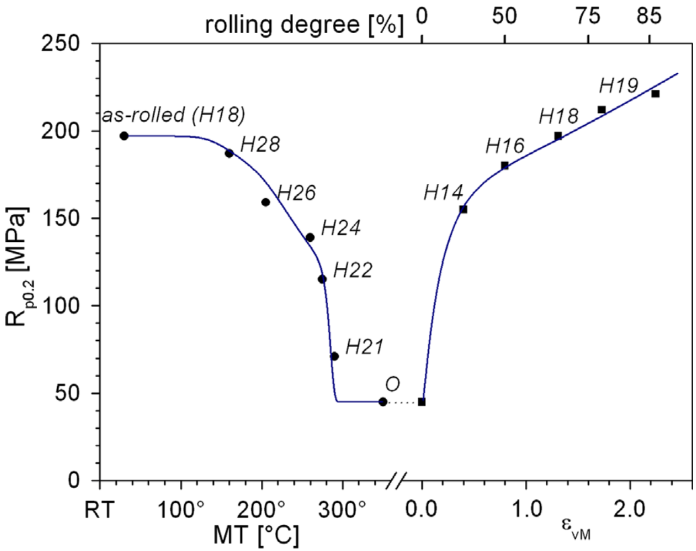
\includegraphics[width=0.45\textwidth]{media/cold-working.png}
\end{wrapfigure}

\phantom{}

\subsection{Cold-working H}
In Hx$n$, where $n=[1,9]$, x:

\begin{tabular}{|c|l|}
  \hline \textbf{x} & \textbf{Meaning}\\
  \hline x=1 & cold-worked\\
  \hline x=2 & \makecell[l]{cold-worked and partially annealed\\for improved temperature resistance}\\
  \hline x=3 & \makecell[l]{cold-worked and stabilization-annealed\\to prevent aging at room temperature}\\
  \hline x=4 & cold-worked and varnished + blacked\\
  \hline 
\end{tabular}
\wrapfill
\vspace*{-10cm}

\newpage
\subsection{Precipitation hardening (Age hardening)}
\subsubsection{Age hardening steps}
\begin{enumerate}
  \item \textbf{Solution annealing (W)}: dissolves existing precipitates in the alloy
  \item \textbf{Quenching}: rapidly cools to form a supersaturated solid solution without precipitates
  \item \textbf{Aging}: small, coherent precipitates form, strengthening the alloy
\end{enumerate}

\subsubsection{Aging types}
\begin{table}[ht!]
  \centering
  \begin{tabular}{|l|l|l|}
    \hline \textbf{Type} & \textbf{Temperature} & \textbf{Properties}\\
    \hline Natural aging & Room temperature & Moderate strength, lower hardness, higher ductility\\
    \hline Artificial aging & Elevated temperature (120-200$^\circ$C) & higher strength and hardness, lower ductility\\
    \hline 
  \end{tabular}
\end{table}

\subsubsection{Graph representation}
T1 to T8 process paths are visible in section 14.2, table 14.2.3.

\begin{figure}[ht!]
  \centering
  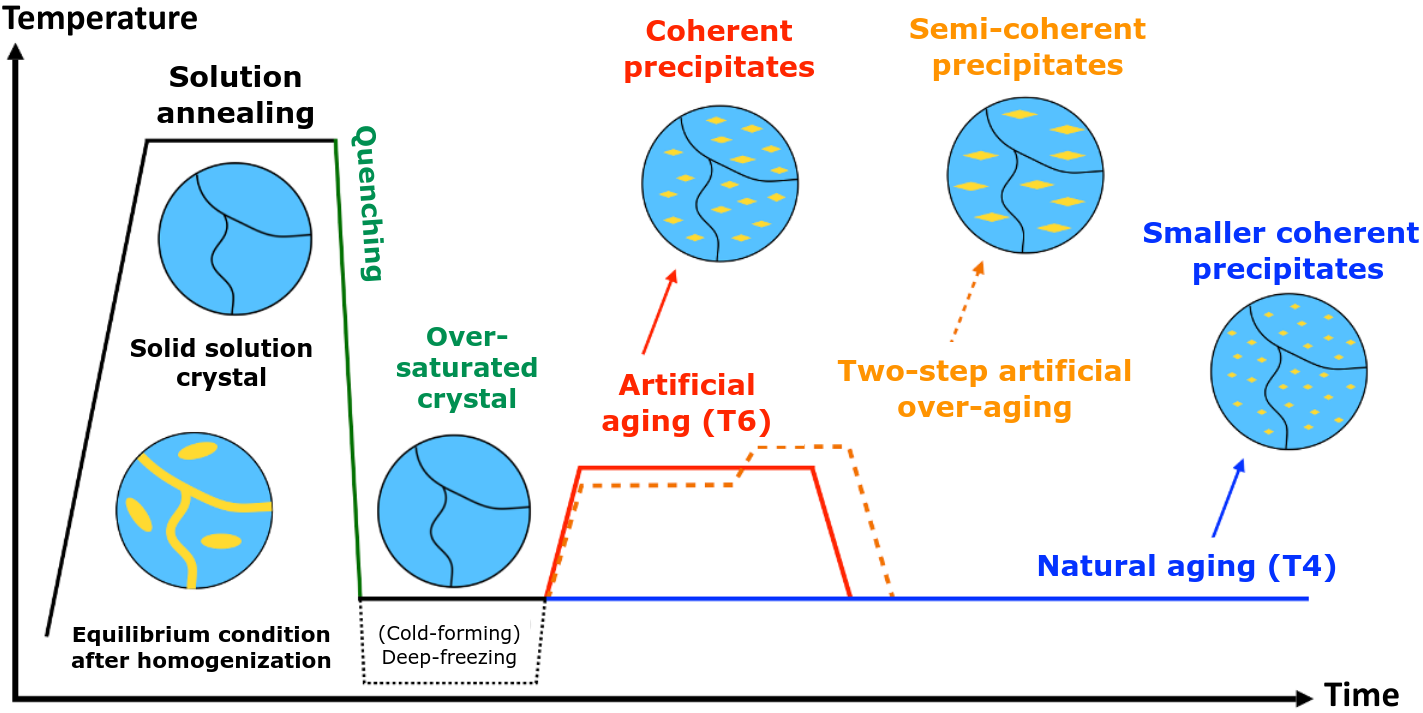
\includegraphics[width=.9\textwidth]{media/aging.png}
\end{figure}

\subsection{Lattice coherency of precipitates}
\begin{itemize}
  \item \textbf{Coherent precipitates}: Lattice planes align perfectly, and elastic distortions extend deep into the surrounding crystal. These distortions act as strong barriers to dislocation movement, resulting in a significant increase in strength
  \item \textbf{Semi-coherent precipitates}: Partial lattice mismatch causes dislocations at the interface, reducing elastic distortion and strength compared to coherent precipitates
  \item \textbf{Incoherent precipitates}: Lattice planes are misaligned and incompatible with the matrix, producting little to no elastic distortion and minimal strengthening effect
\end{itemize}

\begin{figure}[ht!]
  \centering
  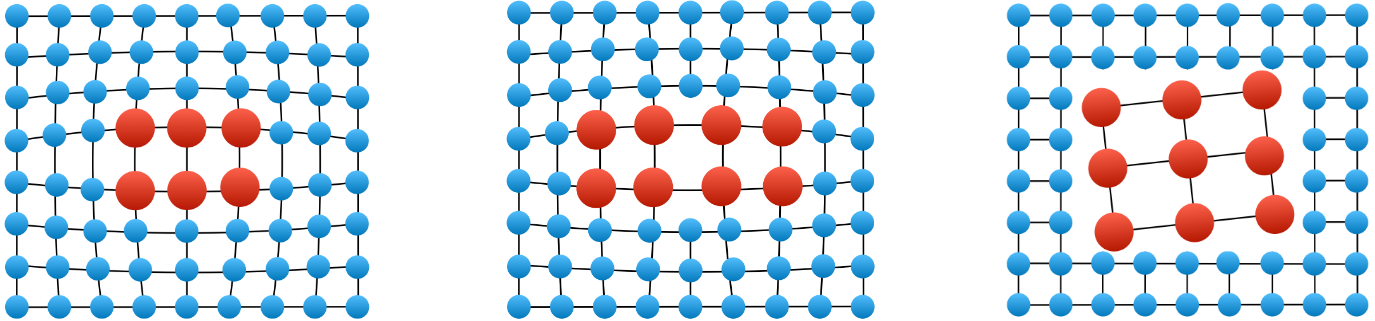
\includegraphics[width=.95\textwidth]{media/lattice_coherency.png}
  \caption*{Coherent (left), Semi-coherent (middle), Incoherent (right)}
\end{figure}

\newpage
\subsection{Precipitation hardening: Artificial aging}
Material strength rises with the formation of coherent precipitates and reaches its
maximum when tey are finely dispesed. Over-aging leads to loss of coherency and reduced
strength.

\begin{figure}[ht!]
  \centering
  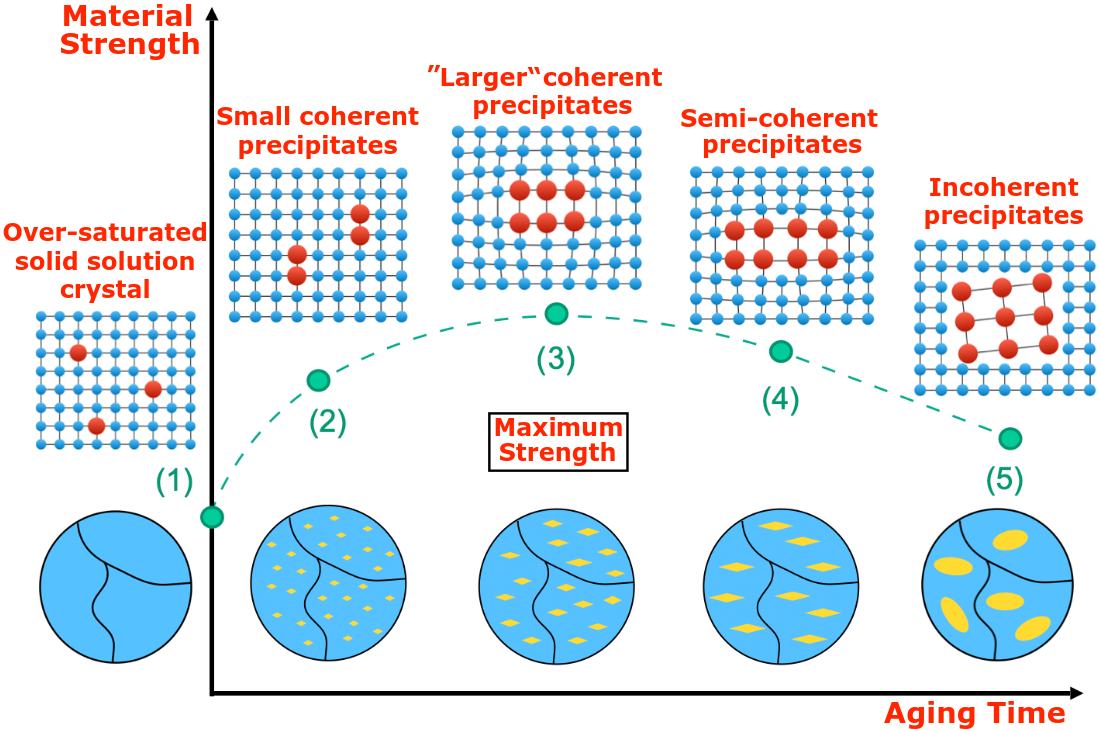
\includegraphics[width=.8\textwidth]{media/artificial_aging.png}
  \caption*{Artificial aging of EN AW-2024 (similar to 6000 and 7000 alloys)}
\end{figure}

\subsection{Precipitates in aluminum alloys}
\begin{itemize}
  \item Precipitates are plate- or disc-shaped, observable under transmission electron microscopy (TEM)
  \item Coherent GPII zones are metastable and maintain lattice alignment with the matrix
  \item Fully stable precipitates become larger and incoherent, leading to over-aging and reduced strength
\end{itemize}

\subsubsection{Precipitation hardening in Aerospace}
Process overview of a sheet metal ribs in the horizontal stabilizer of the PC-12 aircraft (EN AW-2024 / AlCu4Mg1)
\begin{enumerate}
  \item Solution annealing and quenching: material becomes soft
  \item (Optional) Deep freezing for storage or transport to prevent premature aging
  \item Cold forming using a hydrostatic press with a single-piece die
  \item Natural aging at room temperature for approximately 4-5 days, final condition: EN AW-2024-T42
  \item Surface treatment: chromating, priming, and painting.
\end{enumerate}

\newpage
\section{Aluminum Wrought Alloys}


\newpage
\appendix
\printacronyms[name=Glossary, heading=section]
\newpage
\renewcommand\nomgroup[1]{%
  \item[\bfseries
  \ifstrequal{#1}{M}{Elastic moduli}{%
  \ifstrequal{#1}{S}{Strength measures}{%
  \ifstrequal{#1}{D}{Ductility measures}{%
  \ifstrequal{#1}{R}{Ratios}{}}}}%
]}

% Elastic moduli
\nomenclature[M01]{$E$}{Young's modulus}
\nomenclature[M02]{$G$}{Shear modulus}

% Strength measures
\nomenclature[S01]{$R_{\text{p}0.2}$}{0.2\% yield strength}
\nomenclature[S02]{$R_\text{eH}$}{Upper yield point}
\nomenclature[S03]{$R_\text{m}$}{Tensile strength}

% Ductility measures
\nomenclature[D01]{$A_\text{g}$}{Uniform strain}
\nomenclature[D02]{$A$}{Fracture strain}
\nomenclature[D03]{$A_n$}{Elongation measured with \ensuremath{\dm L_0 = n\sqrt{S_0}}}

% Ratios
\nomenclature[R01]{$\nu$}{Poisson's ratio}
\vspace*{-1cm}
% makeindex Materials-lab.nlo -s nomencl.ist -o Materials-lab.nls
\printnomenclature

\end{document}
